\documentclass[aps,onecolumn,twoside,secnumarabic,balancelastpage,amsmath,amssymb,nofootinbib,hyperref=pdftex]{revtex4}


\usepackage{color}         % produces boxes or entire pages with colored backgrounds
\usepackage{multirow}
\usepackage{graphics}      % standard graphics specifications
\usepackage[pdftex]{graphicx}      % alternative graphics specifications
\usepackage{longtable}     % helps with long table options
\usepackage[english]{babel}
\setlength{\parskip}{1em}
\usepackage{amsmath}
\usepackage{epsf}          % old package handles encapsulated post script issues
\usepackage{bm}            % special 'bold-math' package
\usepackage{verbatim}			% for comment environment
\usepackage[colorlinks=true]{hyperref}  % this package should be added after all others % use as follows: \url{http://web.mit.edu/8.13}                                    
                                  

\begin{document}
\title{}
\author         {Noah Steinberg}
\email          {nastein@umich.edu}
\date{\today}
\affiliation{University of Michigan - Physics}

\maketitle

\tableofcontents

\section{ Three photon search \tiny{3/26/20}}

The two most relevant papers for this three photon search at the moment are \cite{Chawdhry:2019bji} and \cite{Aaboud:2018djx}. Ref.\cite{Chawdhry:2019bji} describes the calculation and comparison to experiment of $ p p \rightarrow \gamma\gamma\gamma$ at NNLO QCD precision for 8 TeV LHC. This paper contains information on analysis cuts and measured differential cross sections. 
\vskip 0.12in
Ref.\cite{Aaboud:2018djx} describes an analysis looking for pairs of highly collimated photon jets which could come from the decay chain $X\rightarrow aa\rightarrow \gamma\gamma\gamma\gamma$ where $m_{a}/m_{X} \ll 1$, where X and a are scalar particles. 
\vskip 0.12in
We first want to investigate the relationship between the generated $\Delta R$ between photons and the mass of the light higgs. To this end we plot below the smallest $\Delta R$ between two photons in each event, as a function of the ratio $m_{h}/M_{H}$. Since $M_{H}$ = 125 GeV, this is equivalent to using light higgs masses $m_{h}$ = 10 GeV, 1 GeV, 500 MeV, 100 MeV.


\begin{figure}[t]
\begin{center}
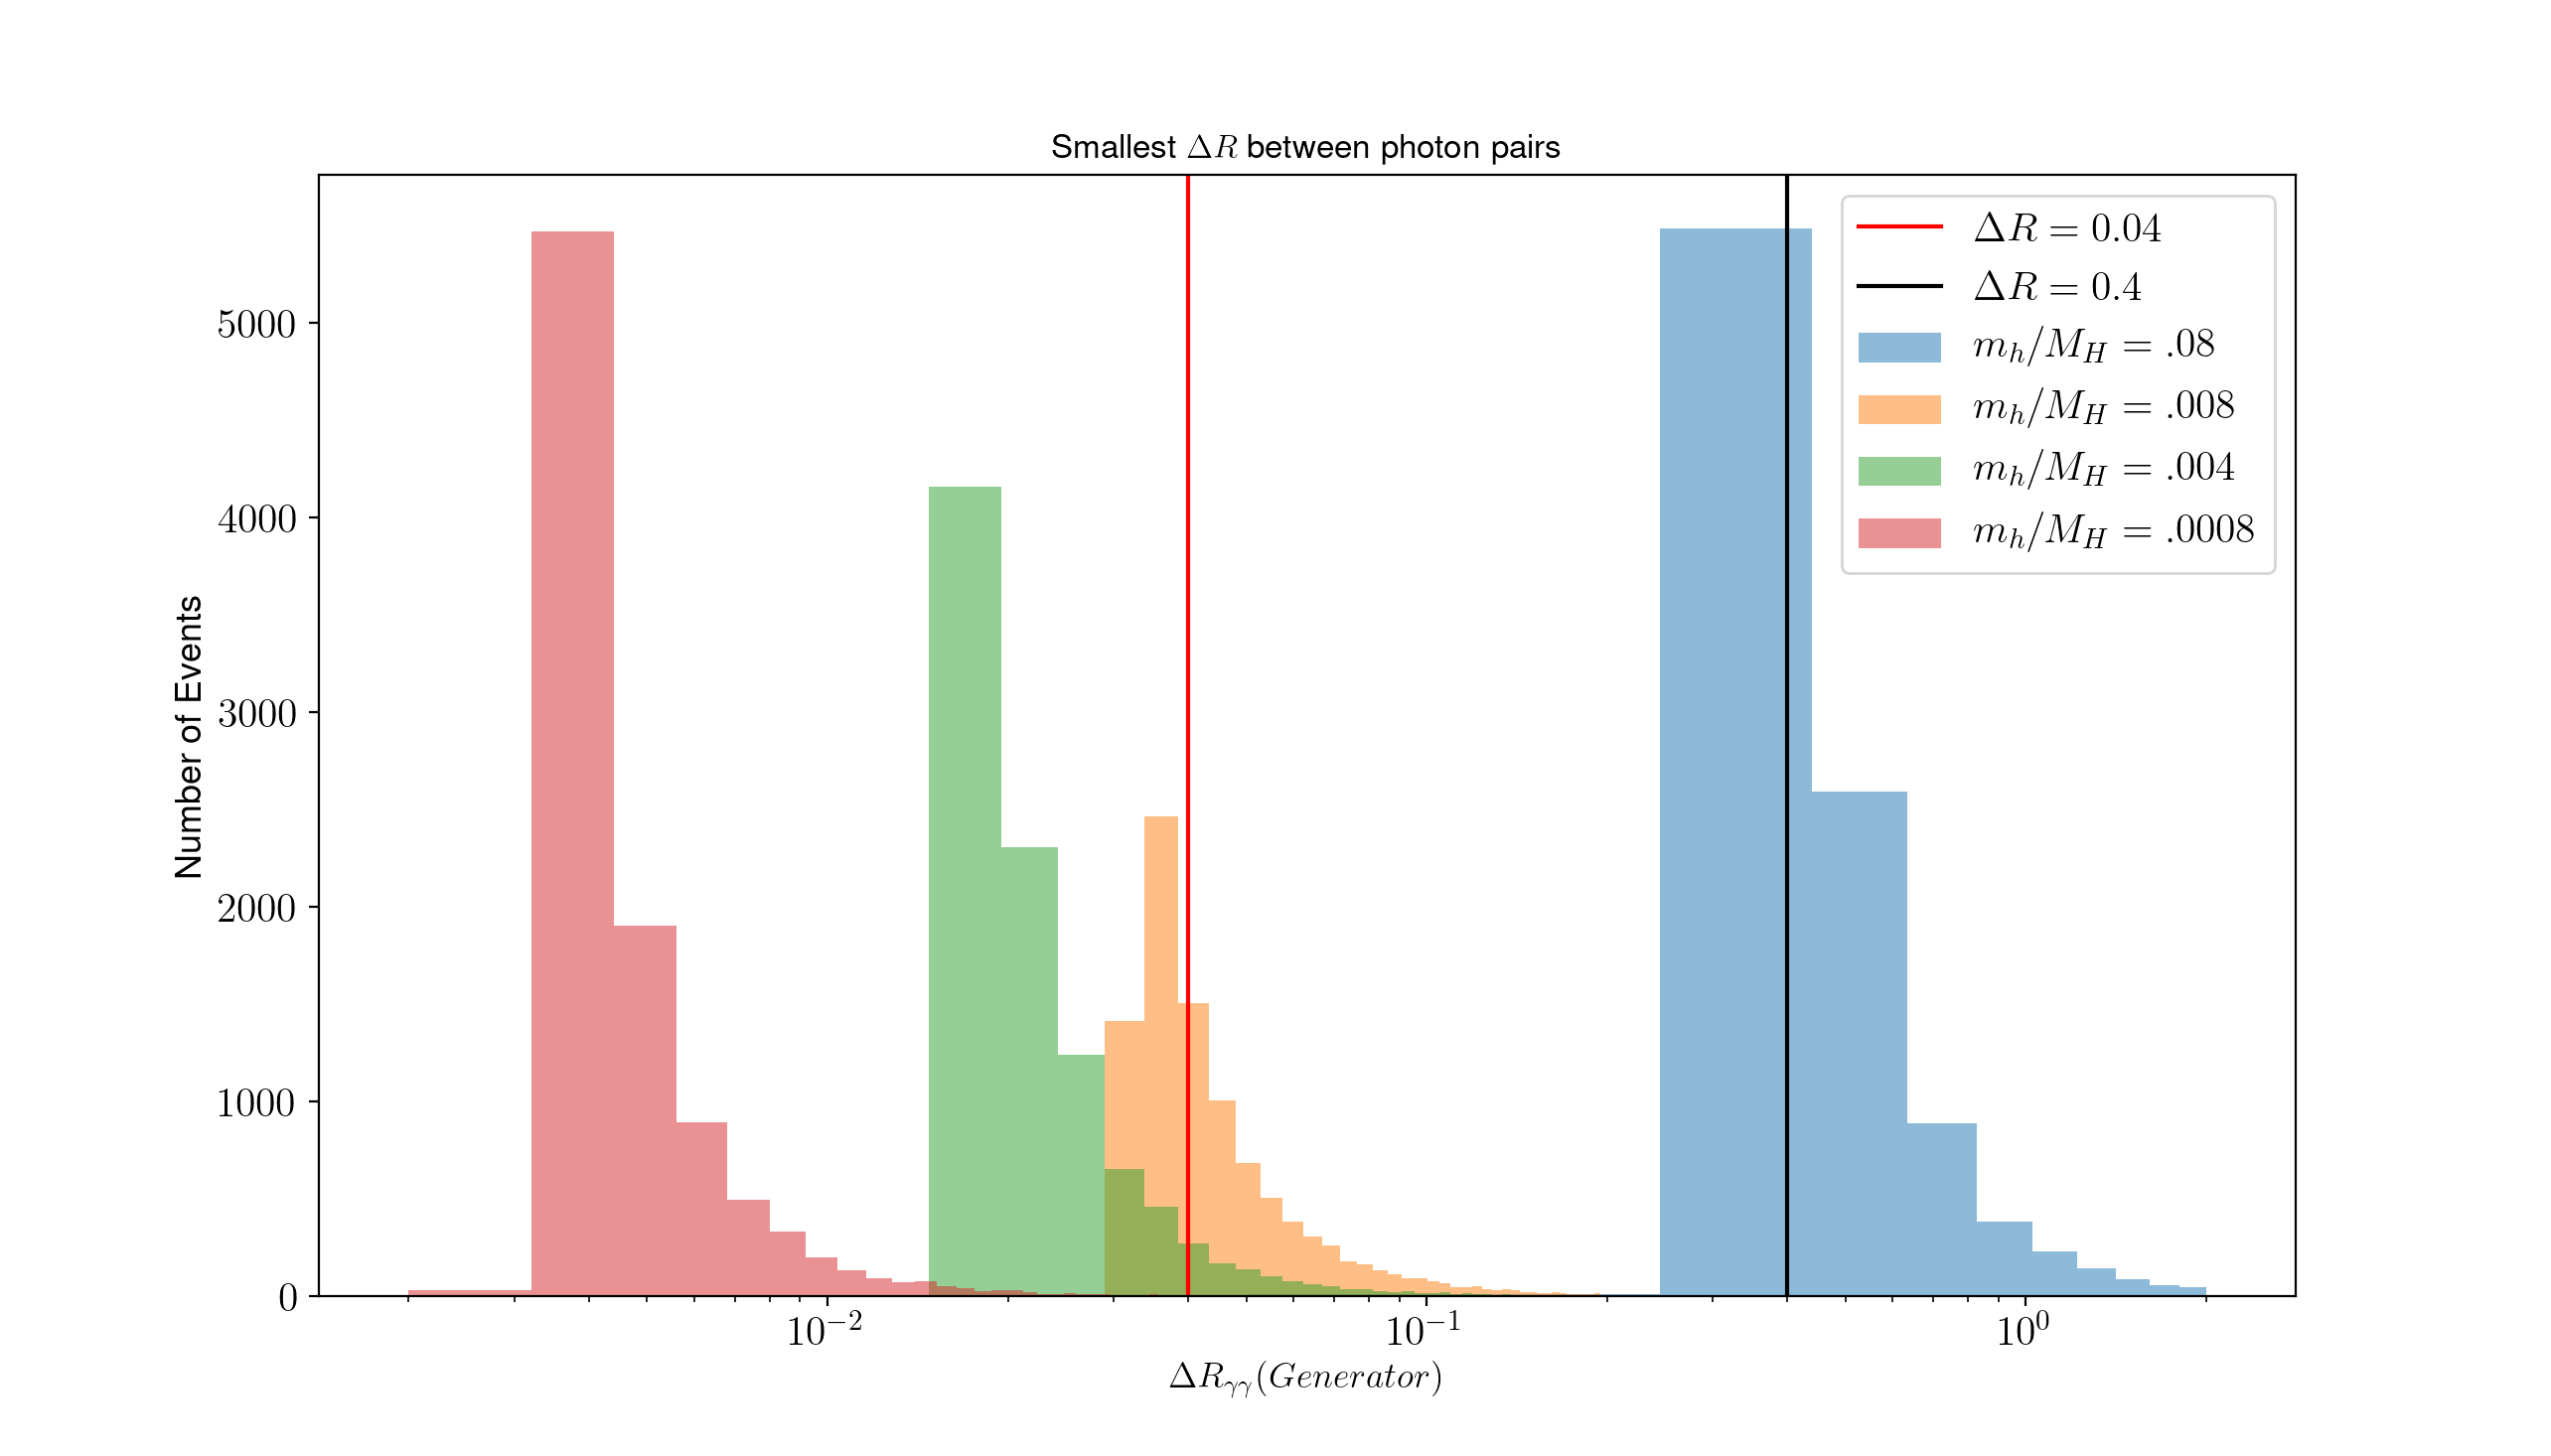
\includegraphics[width=12cm]{deltaRs.png}
\caption{Smallest $\Delta R$ in each event as a function of the ratio $m_{h}/M_{H}$. Smaller ratios (smaller light higgs masses $m_{h}$) lead to more tightly collimated photon pairs (smaller $\Delta R$). Also shown are lines indicating different photon isolation regions. For $\Delta R < 0.04$ photon pairs are reconstructed as a single photon. For $\Delta R > 0.4$ photon pairs are reconstructed as two separate photons.}
\label{fig:1}
\end{center}
\end{figure}
As $m_{h}$ decreases, we should expect that the light higgses from the decay $H\rightarrow hh$ are more and more boosted, leading to highly collimated photons from the $h$ decays. This is indeed the case as seen in Figure~\ref{fig:1}. The peak of the $\Delta R$ distribution is at roughly $4\times m_{h}/m_{H}$ which is the same number found in Ref.\cite{Aaboud:2018djx}. For $m_{h}/m_{H} < 0.1$, these $\Delta R$ values are far below the typical isolation requirements found in arXiv:1911.00479, which require isolation cuts of $\Delta R > 0.4$ between photons. This corresponds to values of $m_{h}/M_{h} > 0.1$. Thus the analysis of Ref.\cite{Chawdhry:2019bji} is insensitive to mass ratios smaller than this value. 
\vskip 0.12in
In the range $0.04 < \Delta R < 0.4$ photons will fail isolation cuts and be rejected. For $\Delta R < 0.04$ the final state photons will fall inside the size of a single-photon energy cluster in the ATLAS EM calorimeter. The difficult part of this analysis is that we would need one photon pair to have a large $\Delta R$ so that each photon is separately reconstructed, and the other photon pair to have a very small $\Delta R$ so that it is reconstructed as a single photon. 

\section{ Photon categories \tiny{3/30/20}}
We can define a theoretical object, a $\xi$ jet, which is a pair of photons with $0.04 < \Delta R < 0.4$. These objects will currently not be reconstructed with the algorithms used in \cite{Chawdhry:2019bji} and \cite{Aaboud:2018djx} because they are too collimated to pass isolation cuts, but not collimated enough to hit one calorimeter cell and be reconstructed as a single photon. Depending on the mass of the light scalar Higgs, each event can be categorized by how many photon or $\xi$ objects are present. In Fig.~\ref{fig:2} we have plotted the fraction of total events falling into the following categories: (1 photon + $\xi$ jet, 2 $\xi$ jets, 2 photons, 2 photons + 1 $\xi$ jet, 3 photons, and 4 photons) for four different light scalar masses. Each simulation has 10,000 total $H\rightarrow hh\rightarrow \gamma\gamma\gamma\gamma$ events. When no bar is shown it means that that category occurs less than $1:10^3$ times. 

\begin{figure}[t]
\begin{center}
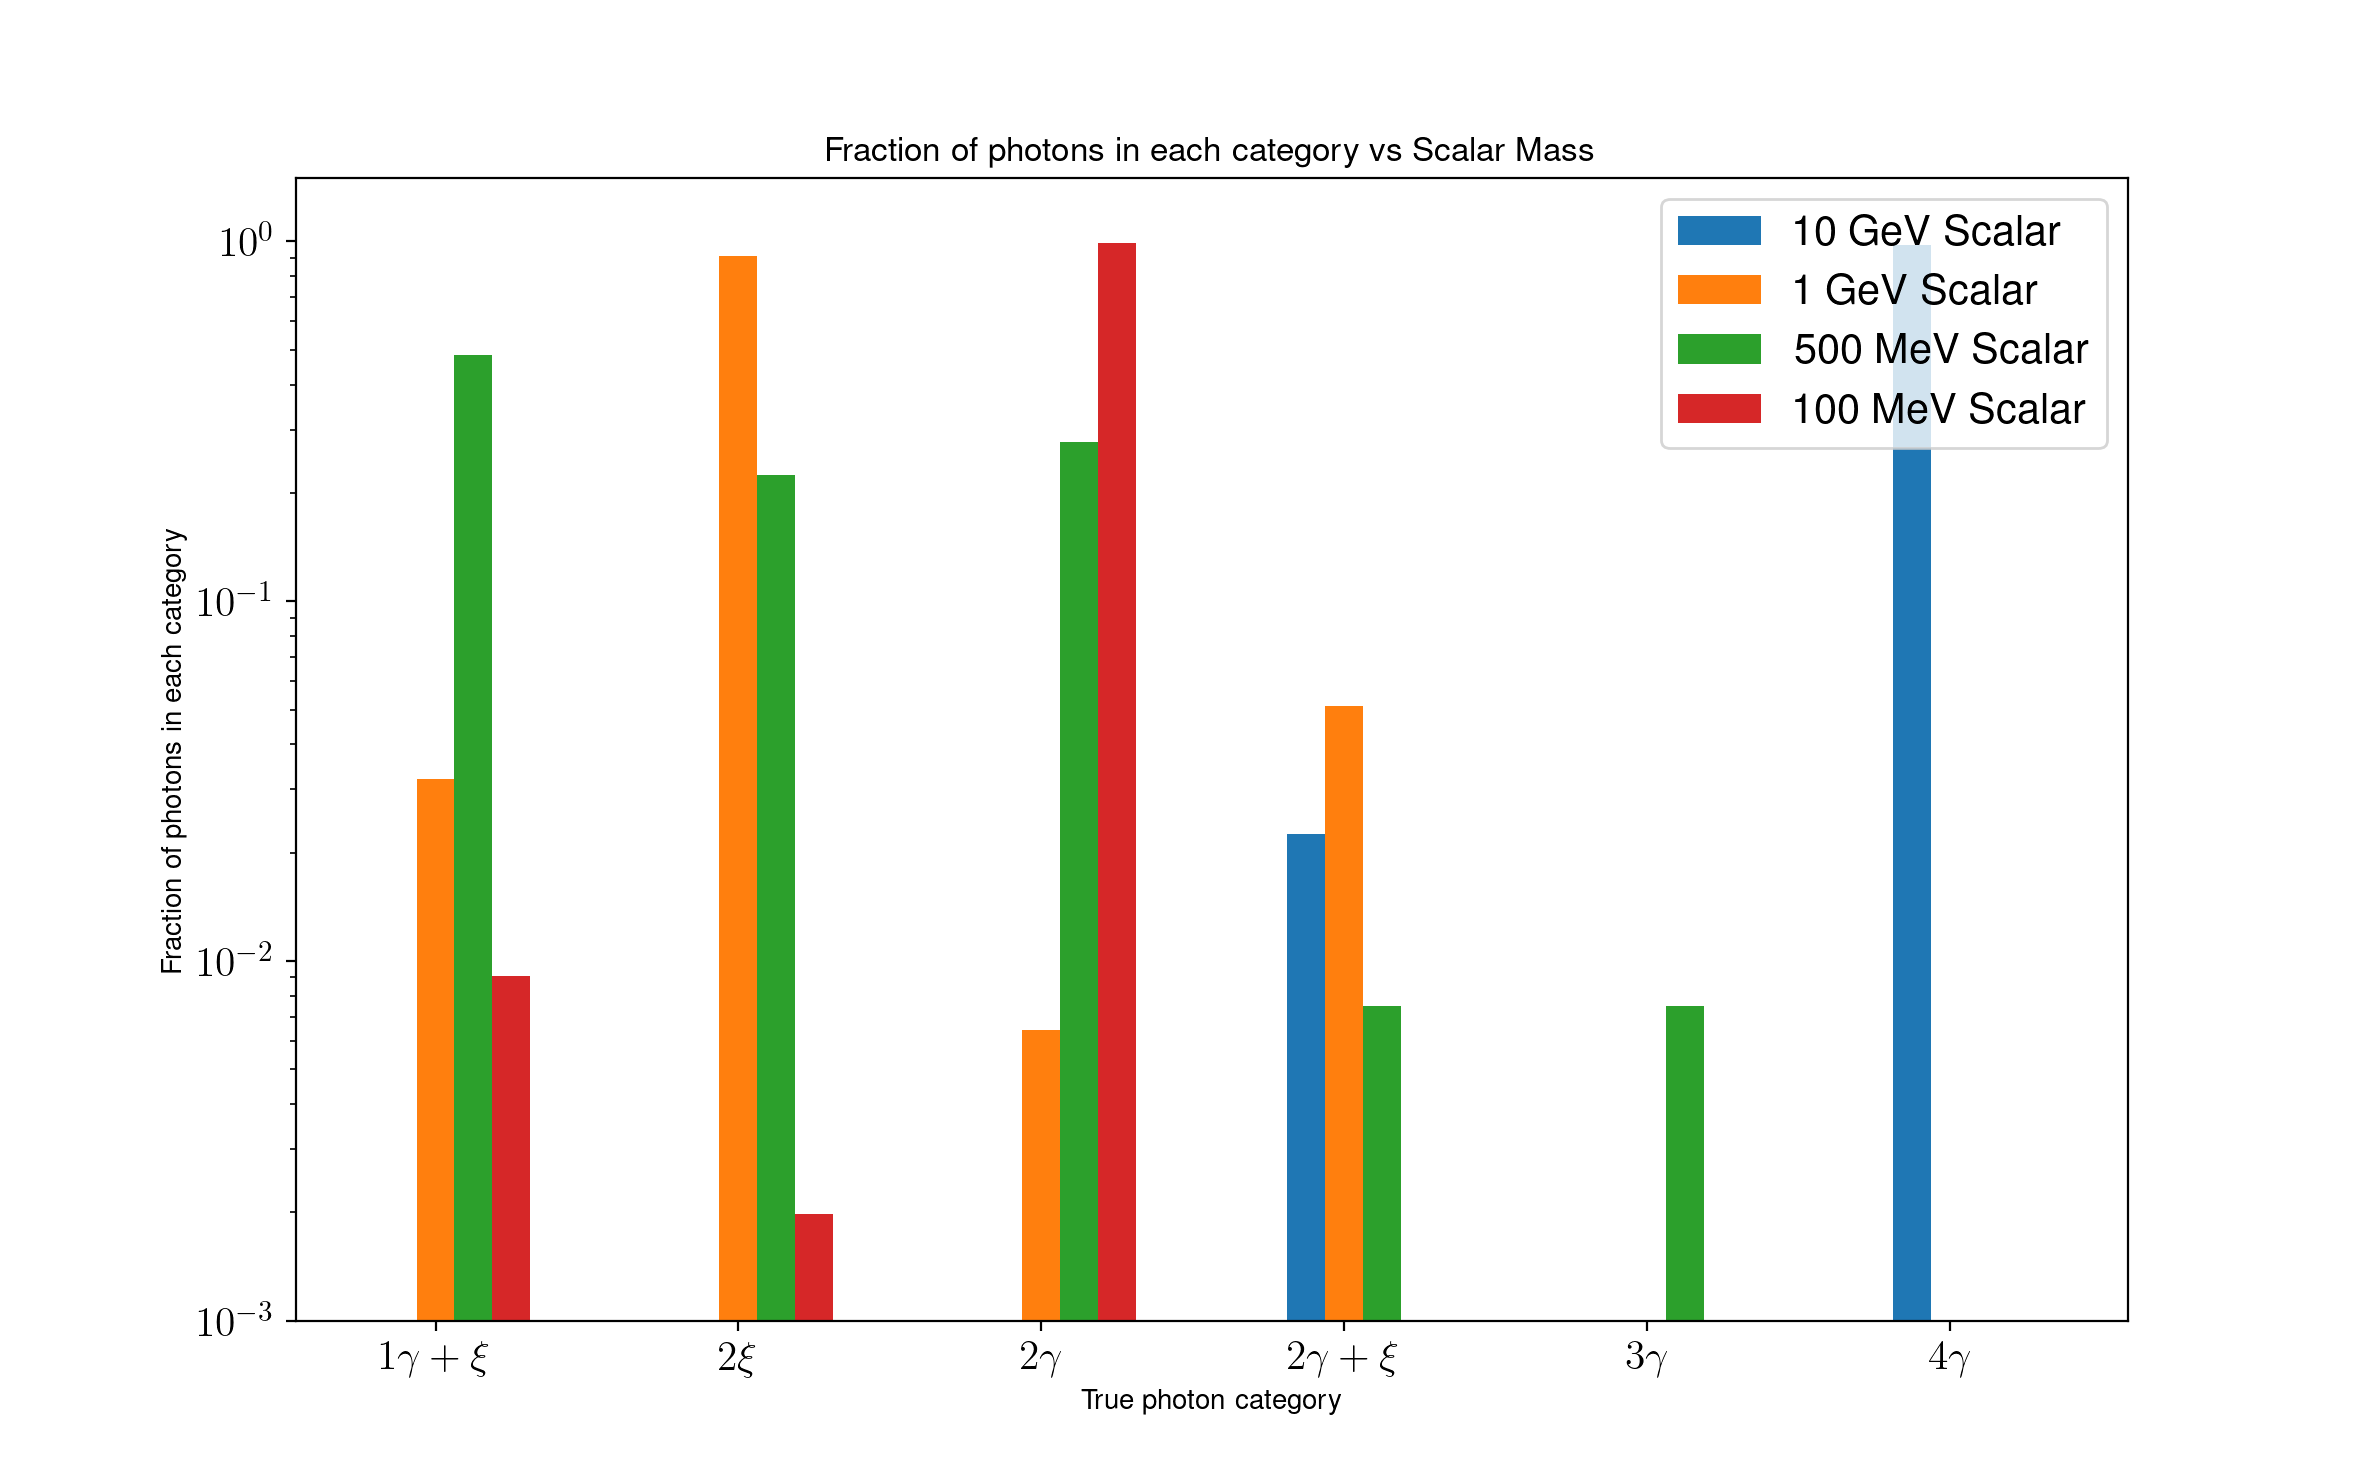
\includegraphics[width=12cm]{photon_fraction.png}
\caption{}
\label{fig:2}
\end{center}
\end{figure}

At large and very small scalar masses (10 GeV and .1 GeV respectively), almost all events fall into the one category with exclusively 4 and 2 photon objects. At 1 GeV a large fraction of the events present with 2 $\xi$ jets but 10\% present as $\xi$ jet with one or two photon objects. For a 500 MeV scalar, events fall broadly into many categories with almost an equal number of events presenting as 1 photon + 1 $\xi$ jet, 2 $\xi$ jets, and 2 photons. Suppressed by an additional $10^{-1}$ are 3 photon events and 2 photons + 1 $\xi$ jet. 

\section{ Anomalous objects \tiny{3/31/20}}
Described in this section is Ref.~\ref{Chakraborty:2017mbz}, where the authors discuss alternative search strategies for "anomalous" objects, hereby meaning objects that are not standard-reconstructed isolated photons, jets, and leptons. Their strategy is to create vetos that eliminate all standard-objects up to e pre-determined acceptance rate. Thus events containing at least one anomalous object (object that pass all of these vetoes) can be identified. In more detail their strategy is as follows 

\begin{enumerate}
\item  Find reconstructed objects by using a single algorithm and a single set of clustering parameters (contains standard and anomalous objects).
\item Map each reconstructed object to a set of chosen variables. Train MVA to identify patches in this multidimensional space occupied by standard objects.
\item Construct vetoes that block these patches rich in standard objects. Vetoes require target-rates, rates at which standard objects will be acceptable. 1\% QCD-jet rate means the boundary is set so that 1\% of QCD jets pass.
\item Objects that pass through all these vetoes are labeled anomalous objects and can become candidate events due to NP and be recorded.
\end{enumerate}
The analysis uses 'Jets' to be the common construct for all physics objects that deposit energy in the calorimeters. Note the distinction between 'jets' and 'QCD jets'. A jet is a generic concept defined in terms of the energy deposits in a calorimeter cell identified by a jet algorithm. When constructing vetoes only the known properties of standard jets are used, no new physics input has been considered.
\vskip 0.12in
Many variables are constructed for each jet including hadronic energy fraction, number of tracks, N-subjettiness, etc.. These variables are used to construct areas in a D-dimensional space that surround standard objects via boosted decision trees. Target rates are set that define the maximum allowed percentage of standard jets that are not vetoed. For example, $R_{j}$, the rate that QCD jets are allowed in at, is .005, meaning that .5\% of QCD jets are not vetoed. Similarly the rate for photons, electrons, and taus are equal and set to $R_{\gamma} = R_{e} = R_{\tau} = 0.05$. 
\vskip 0.12in
Ref.~\ref{Chakraborty}, considers a toy model very similar to ours, with the Higgs coupling to a light scalar which can decay into two photons. They consider a mass of 10 GeV for their light scalar and claim that this mass is sufficient so that the decay products of the light scalar are sufficiently collimated. This seems to be at odds with Fig.~\ref{fig:2} where almost 100\% of decays result in 4 well identified standard photons (though $\mathcal{O}(10^{-2})$ events do result in 2 photons and 1 $\xi$ jet). The trained BDT is used to impose a photon veto region which has efficenies of ~60\% for jets containing two photons (our $\xi$ jets), ~5\% for single photons, and .07\% for QCD-jets. 
\vskip 0.12in
As far as practical matters go, there are to strategies to categorize data. First is an offline analysis. Here we assume that an event has already been triggered through existing trigger options by reconstructing events like muons, electrons, jets, etc.. After the event is saved the anomaly finder tool can be used to look for new physics signatures. The second approach is an online implementation. Here the anomaly finder can be used with existing high level triggers. Ref.~\ref{Chakraborty} claims that ATLAS and CMS have modified their existing trigger menu signficantly by making direct use algorithms and selection criteria similar to offline reconstruction techniques. $Anti-k_{T}$ jets with varying values of jet radius are reconstructed at the HLT,  and identification and tagging the flavor of these jets are now an integral part of the HLT system. These already incorporate advanced MVA. Thus the existing HLT is already efficient enough to handle an algorithm such as the anomaly finder.

\section{Scalar decay length \tiny{4/06/20}}
We can compute the scalar decay length in a simple model described by a scalar with an effective coupling to two photons, $\mathcal{L} = \frac{1}{\Lambda}sF^{\mu\nu}F_{\mu\nu} + \mathcal{L}_{other}$. We are interested in the dependence of the decay length on the mass of the scalar and on the effective cutoff $\Lambda$. 
\vskip 0.12in
In the rest frame of the decaying scalar the partial lifetime to photons is given by
\begin{equation}
\tau(\phi\rightarrow aa) = \frac{16\pi\Lambda^{2}}{m_{\phi}^{3}}.
\end{equation}
We must of course translate this to a lifetime, and then a decay length in the lab frame. Since the scalar will come from a heavy higgs decay with mass $m_{H} = 125 GeV \gg m_{\phi}$, we can approximate the total energy of one of the two scalars to be $E_{\phi} = M_{H}/2$. Thus $\gamma_{boost} = \frac{m_{H}/2}{m_{\phi}}$. This gives a lifetime in the lab frame of
\begin{equation}
\tau_{lab} = \tau(\phi\rightarrow \gamma\gamma)\gamma_{boost} = \frac{8\pi\Lambda^{2}m_{H}}{m_{\phi}^4}.
\end{equation}
In the relativistic approximation $\beta \approx 1 - \frac{1}{2\gamma_{boost}^{2}} = 1 - 2\frac{m_{\phi}^{2}}{m_{H}^{2}}$. This finally leads to a lab decay length of
\begin{equation}
d_{lab} = \beta\tau_{lab} = 8\pi\Lambda^{2}(\frac{m_{H}}{m_{\phi}^{4}})(1 - 2\frac{m_{\phi}^{2}}{m_{H}^{2}}).
\end{equation}
In Fig.~\ref{fig:3} we plot this decay length (in mm) as a function of the light scalar mass, $m_{\phi}$ and the effective cutoff, $\Lambda$.
\begin{figure}[t]
\begin{center}
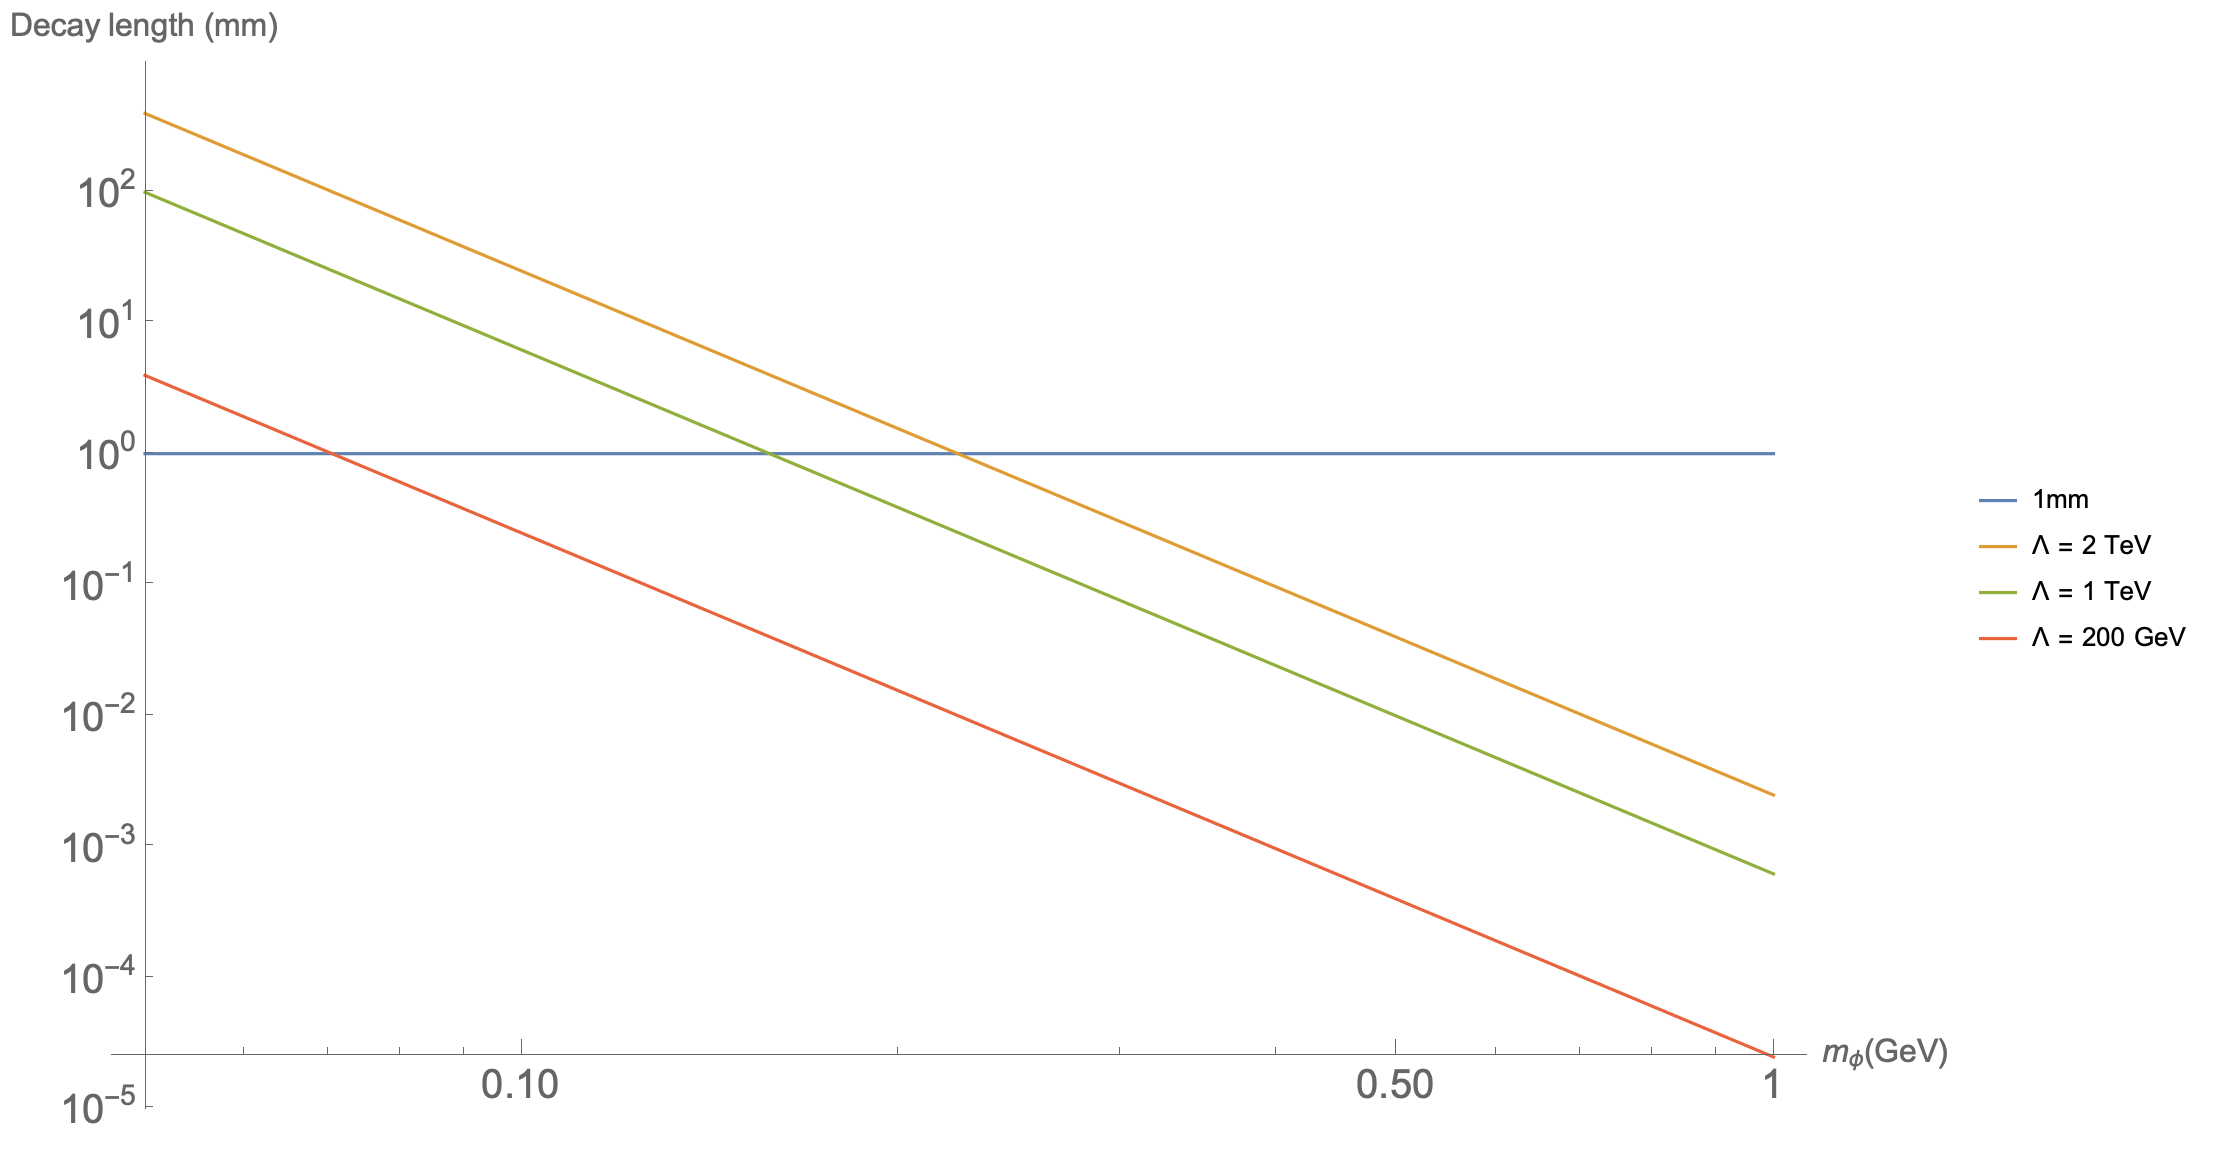
\includegraphics[width=14cm]{decay_length_plot.png}
\caption{Decay length in mm as a function of the light scalar mass, $m_{\phi}$ and the effective cutoff $\Lambda$. Note that both axis are in log scale. The decay length has a quadratic dependence on the cutoff $\Lambda$ as should be expected and increases steeply as $m_{\phi}$ decreases. 1mm decay length is indicated as the blue horizontal line}
\label{fig:3}
\end{center}
\end{figure}
Decay lengths greater than 1mm can lead to displaced vertices and interesting signatures at the LHC. We see for $\Lambda =$ 200 GeV, 1 TeV, 2 TeV that displaced vertices occur for $m_{\phi} \approx$ 70 MeV, 150 MeV, 225 MeV respectively. 
\vskip 0.12in
Fig.~\ref{fig:4} provides a different visualization of this data. We show the cutoff required vs scalar mass for a given decay length. In other words, this shows for a given scalar mass, what cutoff gives the required decay length. We see that larger scalar masses require larger cutoffs for a given decay length.
\begin{figure}[t]
\begin{center}
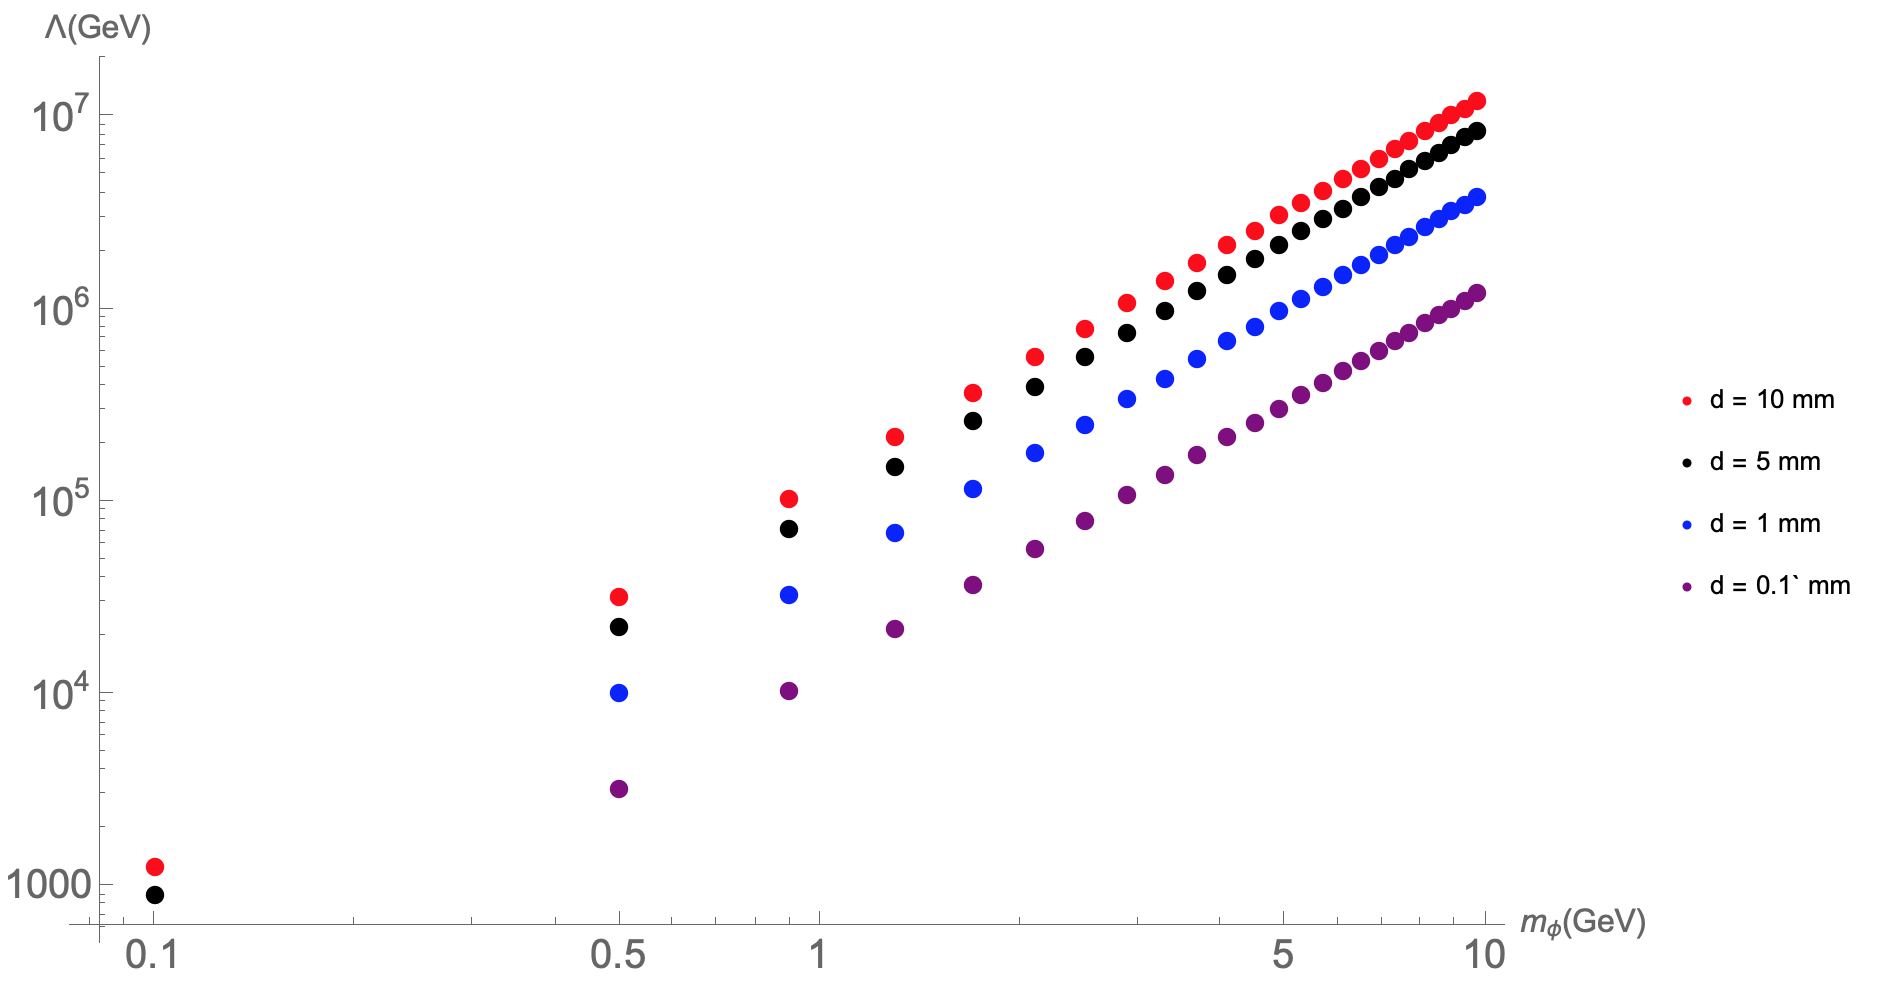
\includegraphics[width=14cm]{mass_vs_lambda.png}
\caption{Required cutoff, $\Lambda$, vs scalar mass, $m_{\phi}$ for a given decay length. Note the log x and y axes.}
\label{fig:4}
\end{center}
\end{figure}

\section{Branching ratio to gauge bosons \tiny{4/17/20}}
We start with the effective lagrangian
\begin{equation}
L =  \frac{1}{\Lambda_{BB}}\phi B^{\mu\nu}B_{\mu\nu} + \frac{1}{\Lambda_{WW}}\phi W^{i\mu\nu}W_{i\mu\nu},
\end{equation}
where $B^{\mu\nu}$ and $W^{i\mu\nu}$ are the hypercharge and SU(2) field strength tensors. Electroweak symmetry breaking mixes the hypercharge and $W^{3}$ component of SU(2) giving the Z boson and photon. So the effective lagrangian in the broken phase is given by
\begin{equation}
L = \phi F^{\mu\nu}F_{\mu\nu}(\frac{c_{w}^{2}}{\Lambda_{BB}} + \frac{s_{w}^{2}}{\Lambda_{WW}}) + \phi Z^{\mu\nu}Z_{\mu\nu}(\frac{s_{w}^{2}}{\Lambda_{BB}} + \frac{c_{w}^{2}}{\Lambda_{WW}}) + 2s_{w}c_{w}\phi Z^{\mu\nu}F_{\mu\nu}(\frac{1}{\Lambda_{BB}} - \frac{1}{\Lambda_{WW}})
\end{equation}
where $F^{\mu\nu}$ and $Z^{\mu\nu}$ are the photon and Z boson field strengths, and $c_{w}$ and $s_{w}$ are the cosine and sine of the weak mixing angle. This effective lagrangian leads to $\phi\rightarrow\gamma\gamma$, $\phi\rightarrow\gamma Z^{*}$, and $\phi\rightarrow Z^{*} Z^{*}$ with off shell Z's for the masses of $m_{\phi}$ we are considering here. The amplitude for the $\phi\rightarrow VV$ transition (where V is a gauge boson) is given by
\begin{equation}
\frac{1}{\Lambda}((\epsilon^{*}_{1}\cdot\epsilon^{*}_{2})(p_{1}\cdot p_{2}) - (\epsilon^{*}_{1}\cdot p_{2})(\epsilon^{*}_{2}\cdot p_{1})),
\end{equation} 
where $p_{1}, \epsilon_{1}$ and $p_{2}, \epsilon_{2}$ are the momenta and polarization vectors of the two gauge bosons, and $\frac{1}{\Lambda}$ stands for whatever linear combination of cutoffs is appropriate for the specific $\phi\rightarrow VV$ decay. After summing over polarizations the squared matrix element is given by
\begin{equation}
|\mathcal{M}|^{2} = \frac{1}{\Lambda^{2}}(2(p_{1}\cdot p_{2})^{2} + p_{1}^{2}p_{2}^{2}).
\label{eq:7}
\end{equation}
\vskip 0.12in
We would like to compute the off shell decay width to pairs of Z bosons and a Z and photon pair. The expression for the decay of a scalar to a pair of off shell vector bosons ($V^{*}V^{*}$) \cite{Djouadi:1995gv} is given by taking the standard formula for the decay width to on shell vectors, and integrating over the invariant masses of of the off shell particles weighted by their propagators. Here we use the narrow width approximation \cite{Uhlemann:2008pm} for the off shell vectors.
\begin{equation}
\Gamma(V^{*}V^{*}) = \frac{1}{\pi^{2}} \int^{m_{\phi}^{2}}_{0} \frac{dQ_{1}^{2}m_{V}\Gamma_{V}}{(Q_{1}^{2} - m_{V}^{2})^{2} + m_{V}^{2}\Gamma_{V}^{2}} \int^{m_{\phi}^{2} - Q_{1}^{2}}_{0} \frac{dQ_{2}^{2}m_{V}\Gamma_{V}}{(Q_{2}^{2} - m_{V}^{2})^{2} + m_{V}^{2}\Gamma_{V}^{2}}\Gamma(VV),
\end{equation}
where $\Gamma_{V}$ and $m_{V}$ are the widths and masses of the vector bosons and $Q_{1}$ and $Q_{2}$ are either invariant masses, and $\Gamma(VV)$ is the decay width to on shell vector bosons with their masses replaced by their invariant masses.
\vskip 0.12in
$\Gamma(VV)$ can be computed by using the feynman rules as shown in Eq.~\ref{eq:7} for off-shell vector bosons. The decay widths are shown as a function of the singlet scalar mass, $m_{\phi}$, below in Fig~\ref{fig:offshell_lifetime}. 
\begin{figure}[htbp]
\begin{center}
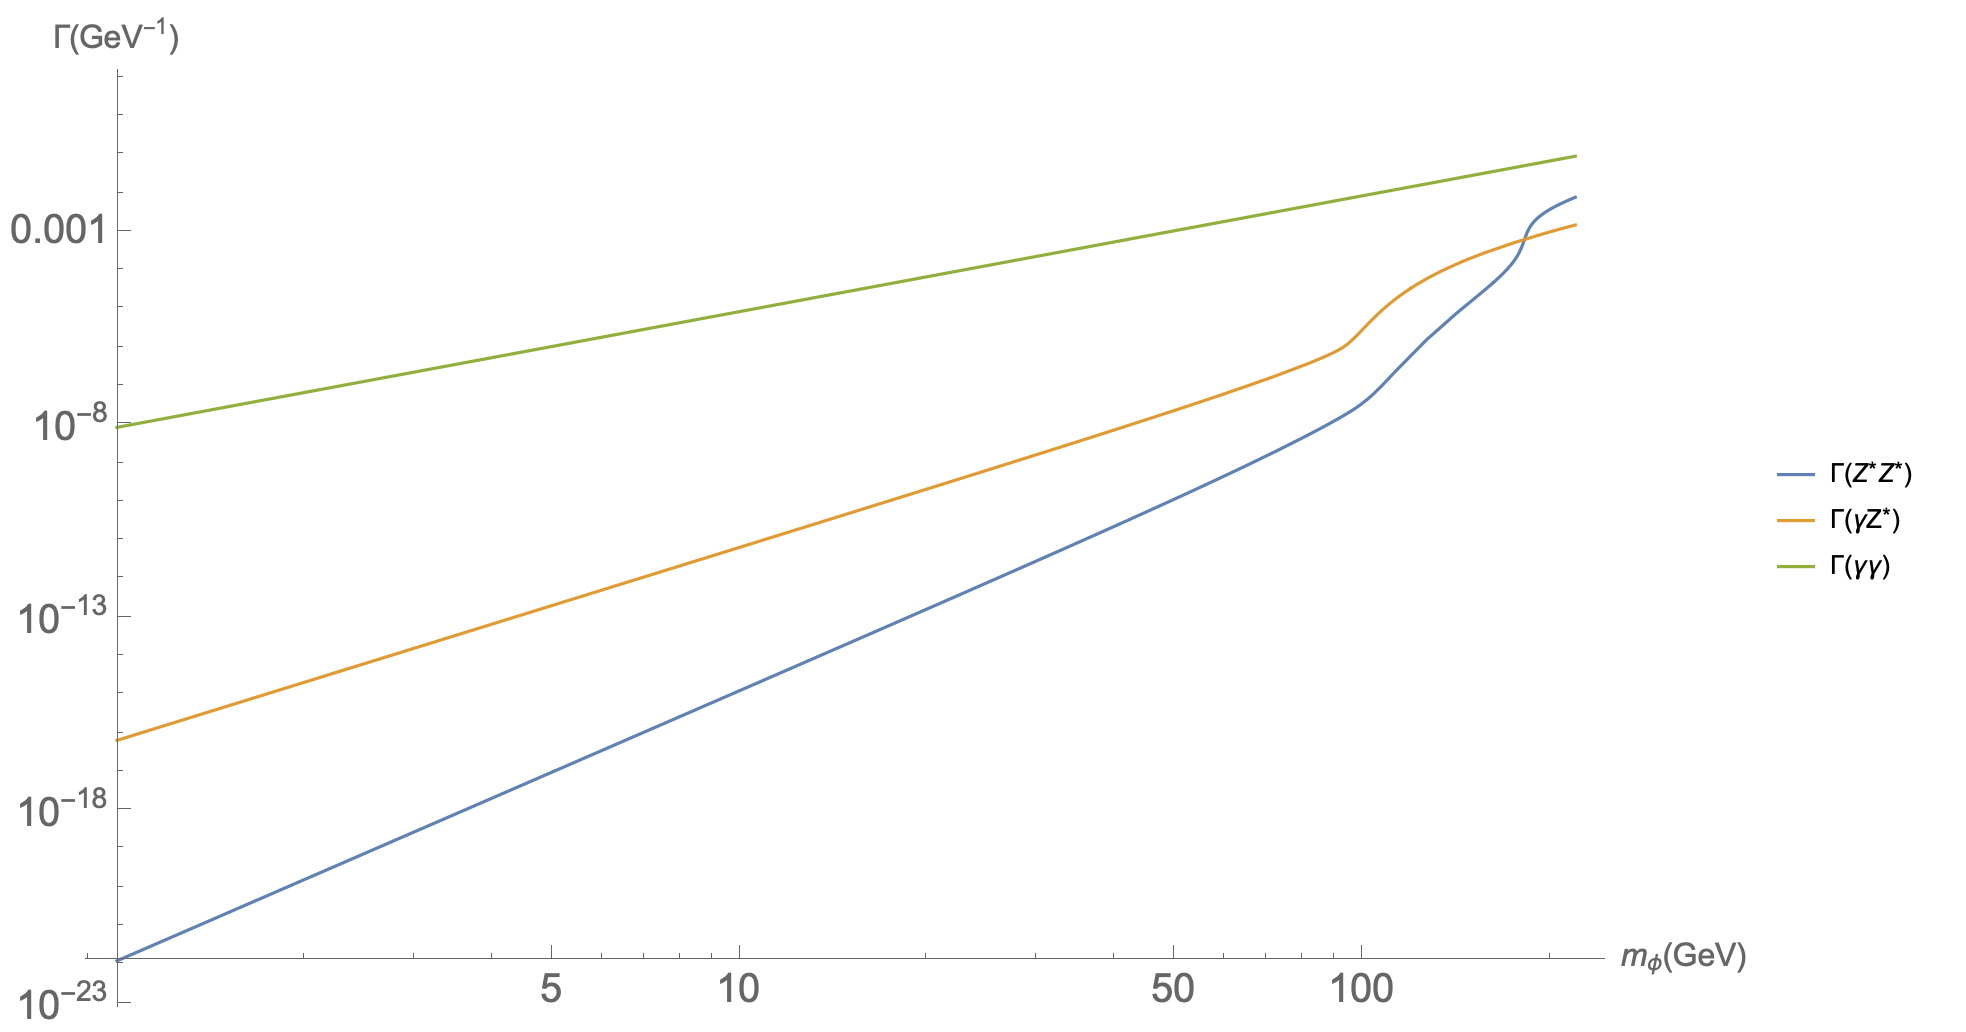
\includegraphics[width=11cm]{offshell_lifetime.png}
\caption{Decay width to Z and $\gamma$ for our toymodel. Here, $\Lambda_{WW} = 1.5$ TeV, and $\Lambda_{BB} = 1$ TeV. One can see that the decay to on shell pairs of photons dominates for the entire range of scalar masses we are interested in. Notice also the thresholds at $m_{\phi} = m_{z}$ and $m_{\phi} = 2 m_{z}$.}
\label{fig:offshell_lifetime}
\end{center}
\end{figure}


\section{Toy Model branching fractions \tiny{4/23/20}}
Here we investigate a toy model extension of the SM involving two additional scalars singlets, $h_{1}$ and $h_{2}$. The lagrangian for these scalars is given by
\begin{equation}
\mathcal{L} = \mathcal{L}_{SM} + \frac{1}{2}(\partial h_{1})^{2} + \frac{1}{2}(\partial h_{2})^{2} - \frac{1}{2}m_{1}^{2}h_{1}^{2} -\frac{1}{2}m_{2}^{2}h_{2}^{2} + \lambda_{2}|H|^{2}h_{1}h_{2}.
\end{equation}
Here $m_{1}$ and $m_{2}$ are the (light) masses of our two scalars, and they enjoy a quartic interaction with the SM Higgs doublet, $H$. No vevs are given to $h_{1}$ and $h_{2}$ and their self interactions are not relevant for this study. The only constraint on $\lambda_{2}$ is from Higgs branching fraction measurements. We study $H$ production and subsequent decay to a pair of light scalars which themselves decay to photons ($ p p > H > h_{1} h_{2} > \gamma\gamma\gamma\gamma)$. Different benchmark points, shown below in Table~\ref{table:bench}, are chosen in this model so as to study what types of photon objects will be produced in these decays.
\begin{table}[htp]
\caption{Benchmark points for toy scalar model. Points are chosen to emphasize unstudied cases of anamolous objects}
\begin{center}
\begin{tabular}{c|c|c}
Benchmark & $m_{1}$ & $m_{2}$\\
A & 1 GeV & 10 GeV\\
B & $10^{-1}$ GeV & 1 GeV\\
C & 1 GeV & 1 GeV\\
D & $10^{-1}$ GeV & 10 GeV\\
\end{tabular}
\end{center}
\label{table:bench}
\end{table}
These points are chosen so that a significant fraction of events are produced with $\xi$ jets and or an odd number of photons). 25000 events are produced for each benchmark point with $\lambda_{2} = 0.1$. Fig.~\ref{fig:toy_model_fractions} shows the fraction of events which fall into each category. 
\begin{figure}[t]
\begin{center}
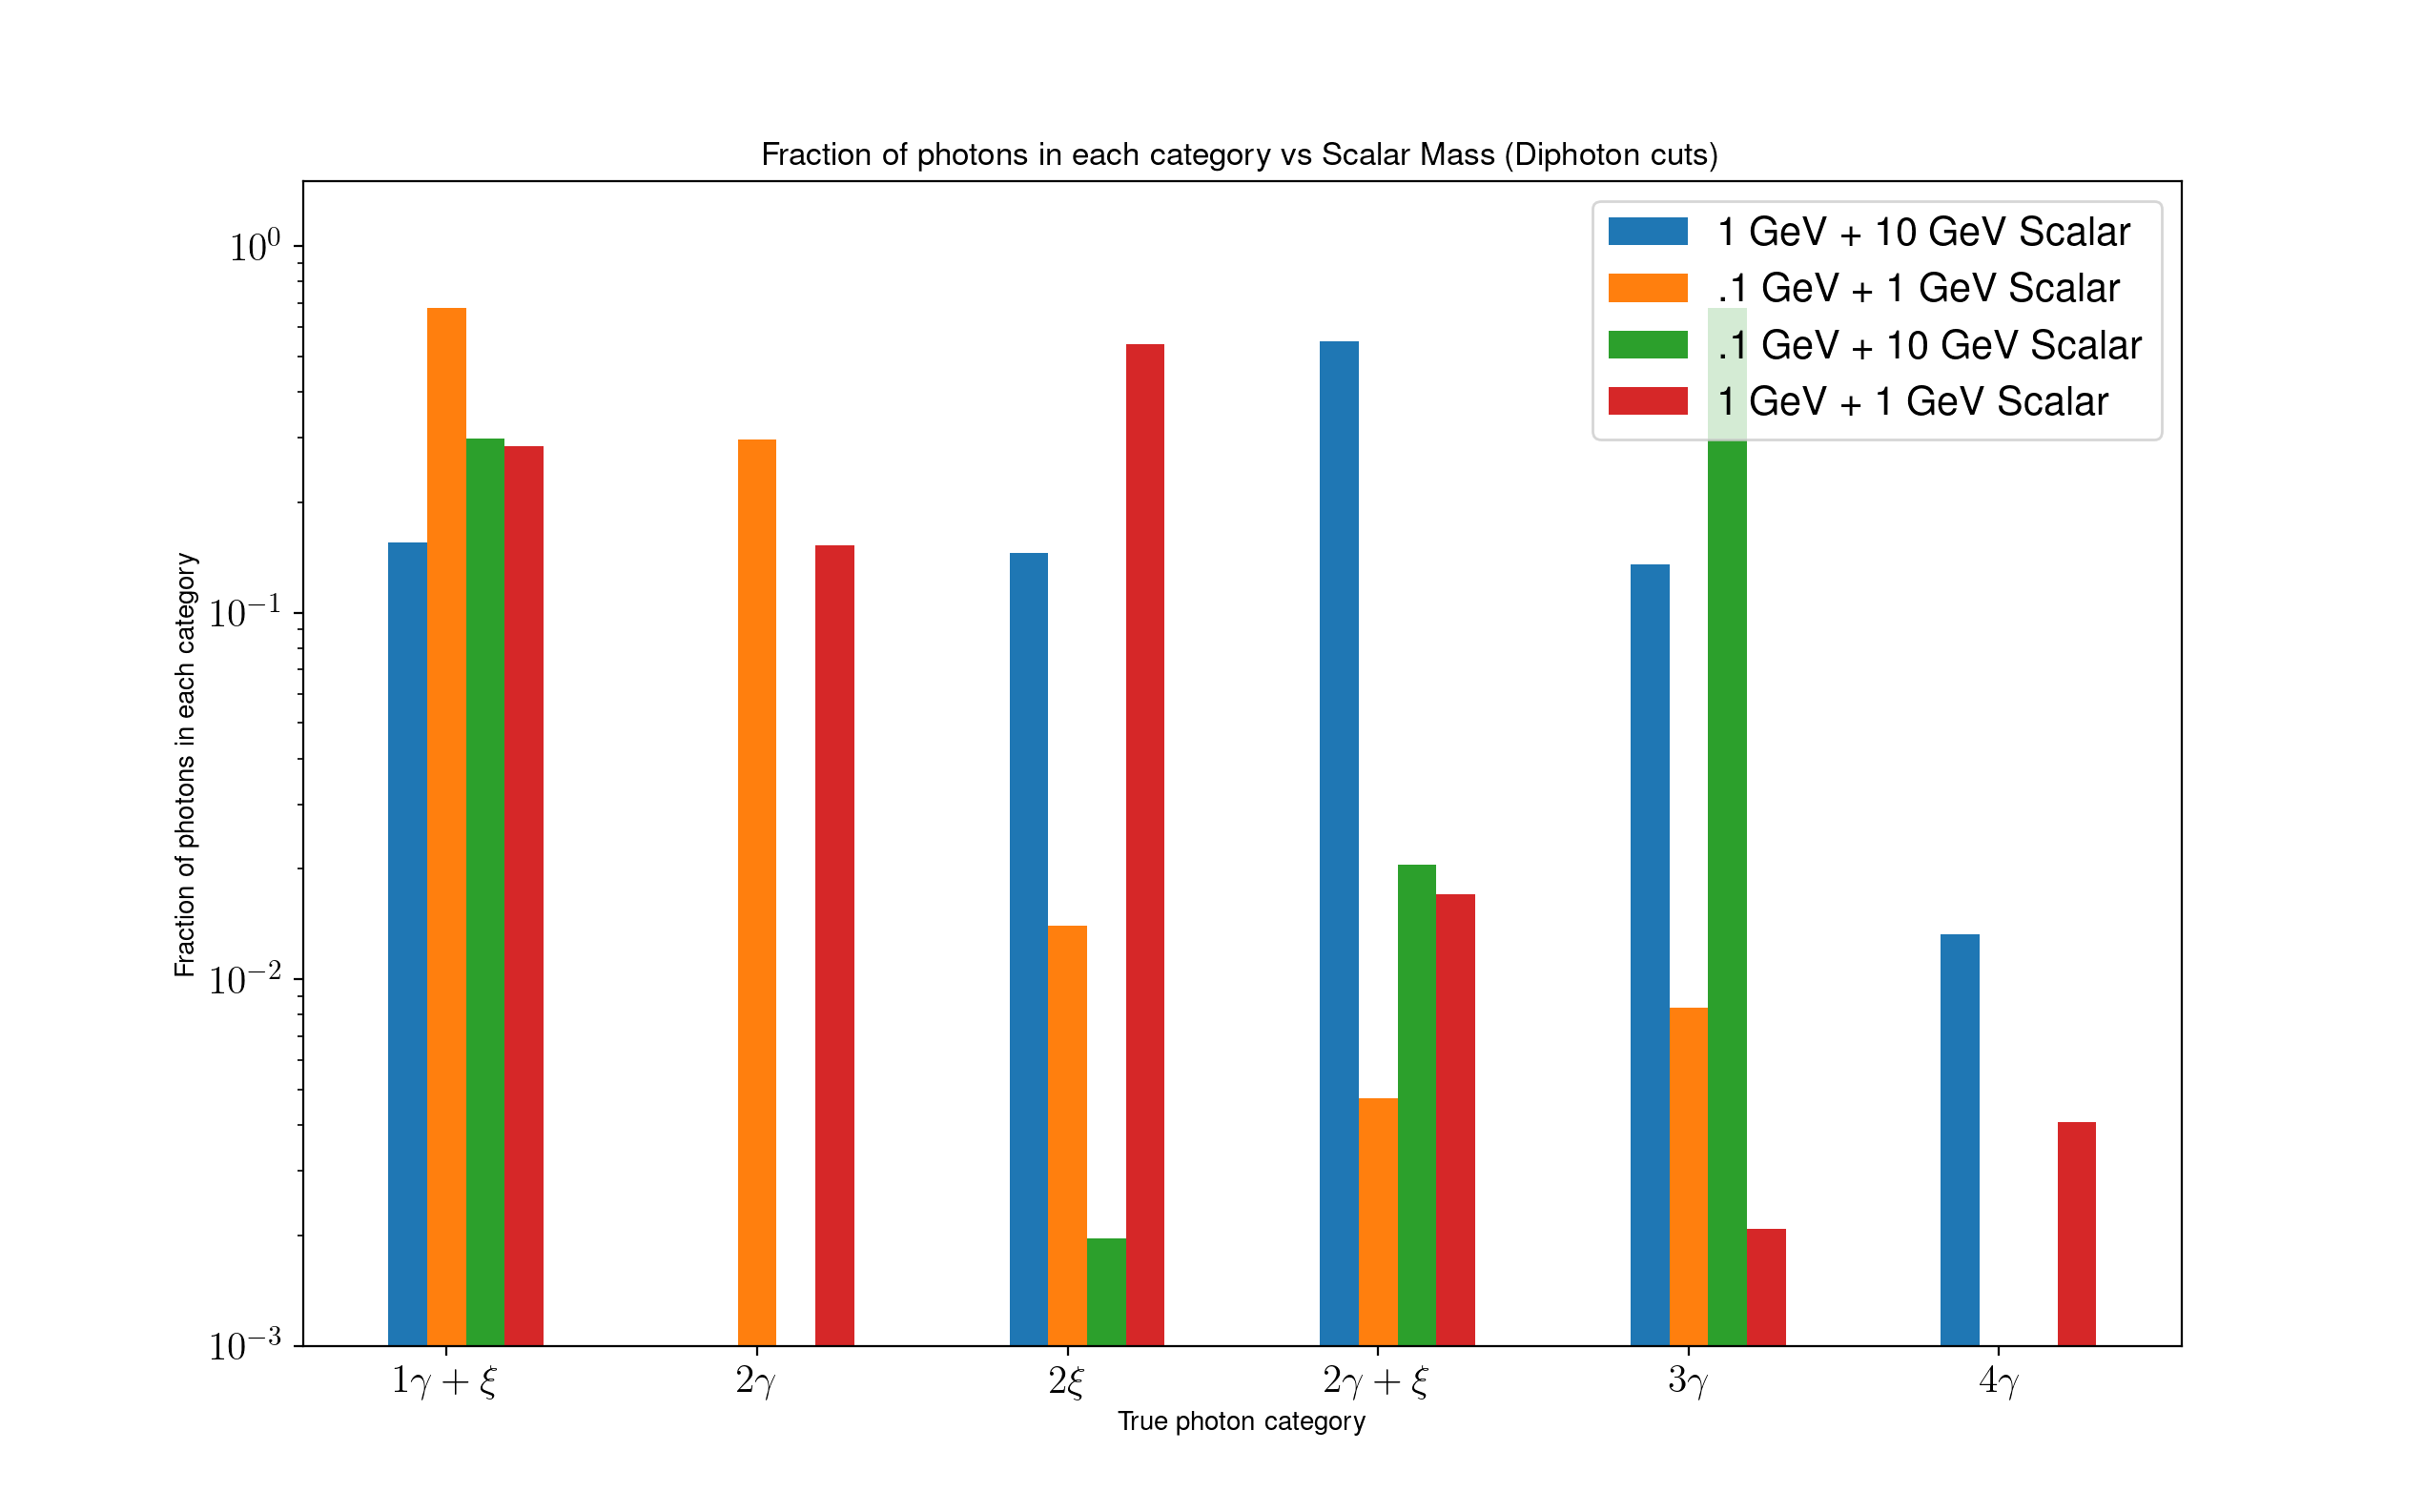
\includegraphics[width=13cm]{toy_model_fractions.png}
\caption{Fraction of photons falling into each category from $ p p > H > h_{1} h_{2} > \gamma\gamma\gamma\gamma)$ events. Four different benchmark masses are chosen for the scalars. No reconstructed cuts have been used.}
\label{fig:toy_model_fractions}
\end{center}
\end{figure}
From the figure we can see that benchmark A most often produces two photons and $1\xi$ jet ($\approx 70\%$) while the remaining events are split roughly equally between $1\gamma + 1\xi$ jet,  $2\gamma s$, and $3\gamma s$. Benchmark B gives mostly $1\gamma + 1\xi$ jet events, while $2\gamma s$ is subdominant. Benchmark C is most striking as the majority of the events produced give a $3\gamma$ signal while $1\gamma + 1\xi$ jet is subdominant. Benchmark D results in $2\xi$ jets $\approx 60\%$ of the time with $1\gamma + 1\xi$ jet and $2\gamma s$ ocurring at rates of $20\%$ and $10\%$ respectively. We summarize these results in Table~\ref{table:dom} below.
\begin{table}[htp]
\caption{Dominant and subdominant photon categories for each benchmark point.}
\begin{center}
\begin{tabular}{c|c|c}
Benchmark & Dominant mode & Subdominant mode\\
A & $2\gamma + 1\xi$ & $1\gamma + 1\xi \approx 2\gamma \approx 3\gamma$\\
B & $1\gamma + 1\xi$ & $2\gamma$\\
C & $3\gamma$ & $1\gamma + 1\xi$\\
D & $2\xi$ & $1\gamma + 1\xi \approx 2\gamma$\\
\end{tabular}
\end{center}
\label{table:dom}
\end{table}
\section{$Z\rightarrow \phi\gamma \rightarrow \gamma\gamma\gamma$ constraints \tiny{5/02/20}}
In our toy model the $Z\phi\gamma$ coupling which gives us offshell $\phi$ decays also leads to the interesting Z decay mode $Z\rightarrow \phi\gamma \rightarrow \gamma\gamma\gamma$. The current upper limit on the $Z\rightarrow \gamma\gamma\gamma$ BR is $2.2\times10^{-6}$ \cite{PDG}. This leads to a constraint on the EFT cutoff. By setting the branching ratio equal to the upper limit, a lower limit on $\Lambda = (\frac{1}{\Lambda_{BB}} - \frac{1}{\Lambda_{WW}})^{-1}$ can be computed as a function of the scalar mass $m_{\phi}$. 
\vskip 0.12in
One should note that below a certain scalar mass the two photons from the $\phi$ decay will be so collimated that the appropriate constraint becomes the 2 photon constraint. The above limits came from the CDF detector at the Tevatron, which has a similar angular resolution for photons as does the LHC\cite{Aaltonen:2012jd}. This means that for $\Delta R < 0.04$, i.e. for scalar masses below $\approx 1$ GeV, the constraint should be the two photon constraint, with an upper limit on the branching ratio of $1.46\times 10^{-5}$. Below in Fig.~\ref{fig:BR_vs_D} we plot the lower limit based on the branching ratio calculation and the upper limit based on the decay length requirement. 

There is in interesting interplay between this lower limit and the upper limit on $\Lambda$ we established before by requiring that the decay of $\phi$ does not lead to displaced vertices at the LHC, i.e. that the decay length is less than 1mm. We can also put an upper limit on $\Lambda$ by requiring that the decay length of our scalar is less than the distance to the ECAL. This distance varies as a function of $\eta$, but in ATLAS at $\eta = 0$ it is 1.5m \cite{eta_ATLAS}.

\begin{figure}[htp]
\begin{center}
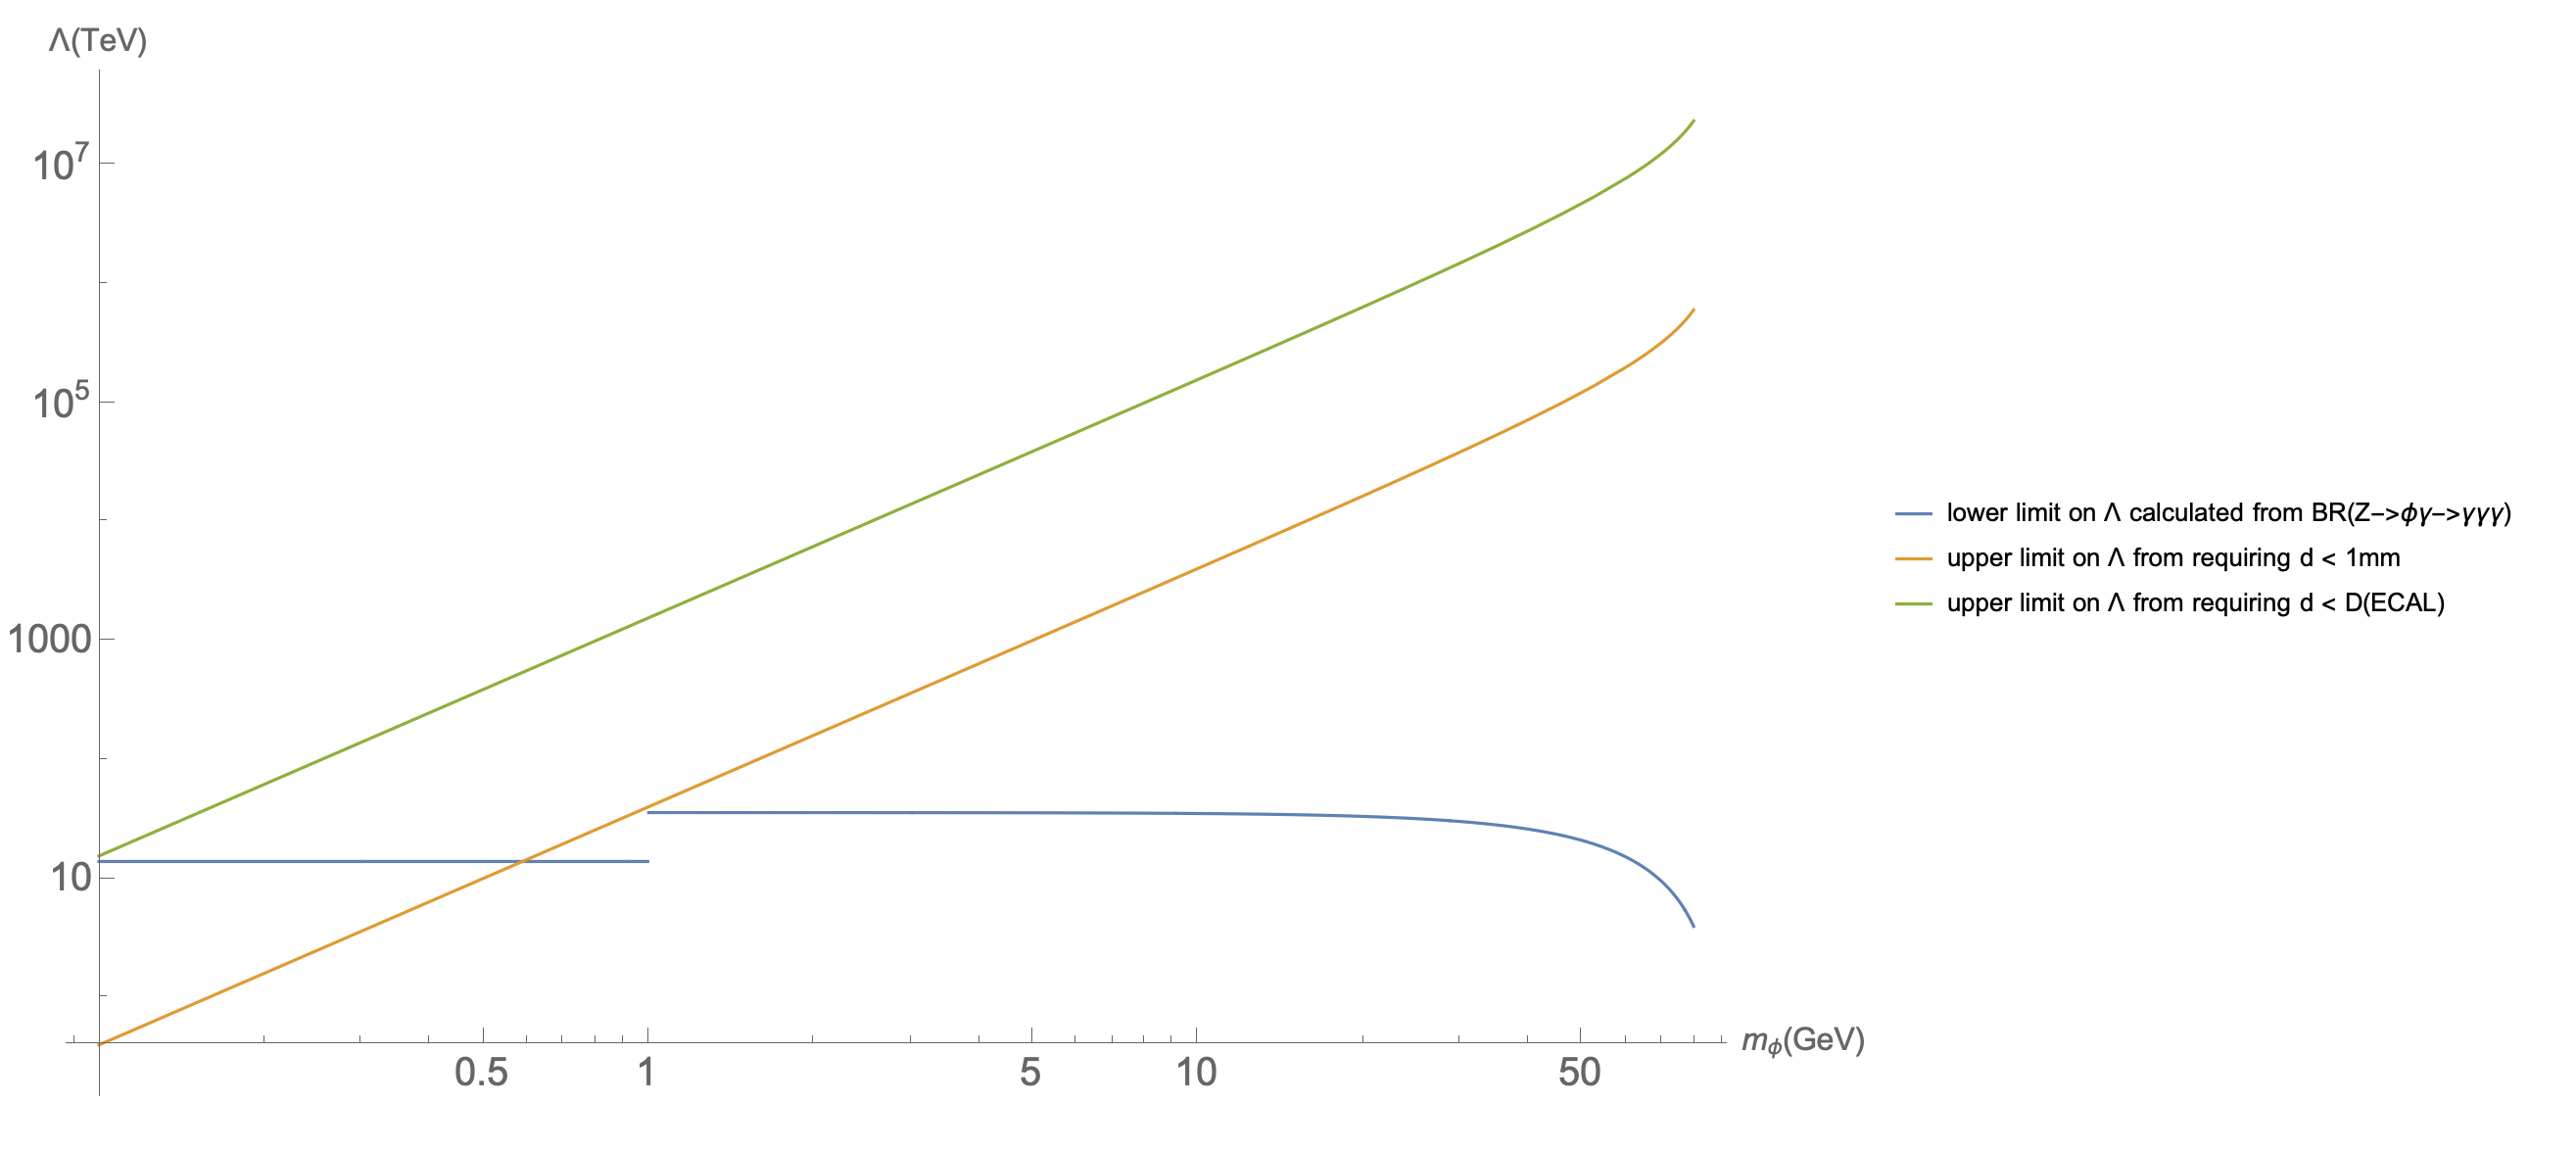
\includegraphics[width=13cm]{BR_vs_D.png}
\caption{Competing limits on $\Lambda$ computed from the  BR($Z\rightarrow \phi\gamma \rightarrow \gamma\gamma\gamma)$ requirement(blue) and from requiring that the decay length be less than 1mm (orange). Note the step down at $m_{\phi} = 1$ GeV comes from using the 2 photon constraint for masses 1 GeV and below, and using the 3 photon constraint for masses above 1 GeV.}
\label{fig:BR_vs_D}
\end{center}
\end{figure}

\section{Reconstructing $\xi$ jets \tiny{5/12/20}}
To reconstruct $\xi$ jets we attempt to follow a similar strategy to as \cite{Ellis:2012zp}. The strategy is as follows. First energy flow (eflow) objects (composed of deposits in calorimeter cells) are clustered into jets using the anti-kt algorithm with $R = 0.25$. Then we re-cluster those energy deposits that were found in each jet using the kt algorithm, this determines a recombination tree for the jets. This tree specifies the subjets at each level of recombination N from N = 1 (the full jet) to N = the number of constituent eflow objects in the jet (no recombination). From here we can compute the N-subjettiness variable for the jet for each N. This variable becomes small when the parameter N is large enough to describe all of the relevant substructure of the jet. It is defined to be
\begin{equation}
\tau_{N} = \frac{\Sigma_{k} p_{T_{k}} \times min[\Delta R_{1,k},\Delta R_{2,k}, . . . , \Delta R_{N,k}]}{\Sigma_{k}p_{T_{k}} \times R},
\end{equation}
where k runs over all the constituents of the jet, $p_{T_{k}}$ is the transverse momentum for the k-th constituent, and R is the characteristic jet radius used in the original jet clustering algorithm. 
\vskip 0.12in
Before applying additional cuts, we would like to characterize the efficiency at which we reconstruct xi jets. To do this we utilize Delphes GenJet objects. GenJets are jets that are clustered, not with calorimeter cells or towers or eflow objects, but with the actual generator level particles. By utilizing GenJets we can define "generated xi jets" and see at what rate we correctly reconstruct these.
\vskip 0.12in
GenJets are clustered with the same strategy as above, first with the anti-kt algorithm with $R = 0.4$, and then reclustered with the kt algorithm. A GenJets is selected as a generated xi jet if it has: 1) At most two photons with PT > 0.5 GeV, 2) no non-photons with PT > 0.5 GeV. Since our theoretical xi jets were defined as pairs of photons with $\Delta R$ between 0.04 and 0.4, we throw out xi jets with $\Delta R < 0.025$ as these will most likely be reconstructed as one photon. 


Once a generated xi jet is identified, we loop over all reconstructed xi jets and attempt to find a matching jet. For reconstructed xi jets, we use at this point our xi-jet 2 definition which is a jet of radius 0.25. Matching is done by comparing the $\Delta R$ between the momentum of the generated and reconstructed jets. If $\Delta R_{gen/reco} < 0.05$ we consider this jet as matched. We also require that the reconstructed xi jets have pass a cut on the required hadronic energy fraction. This cut is that $log(E_{had}/E_{jet}) < -0.8$. As a check we can also compare the PT of the generated and reconstructed jets. These should be very similar unless there are additional hadrons in the jet. Below in Fig.~\ref{fig:gen_reco} we show $\Delta R_{gen/reco}$, which shows the level of matching between generated and reconstructed xi jets, and also as a check that this is independent of our model parameters. In Fig.~\ref{fig:const} we show plots of the $\Delta R$ between the constituents (photons) of our generated xi jets where one can easily see how this quantity shifts as as function of our benchmark points. 

\begin{figure}[t]
\begin{center}
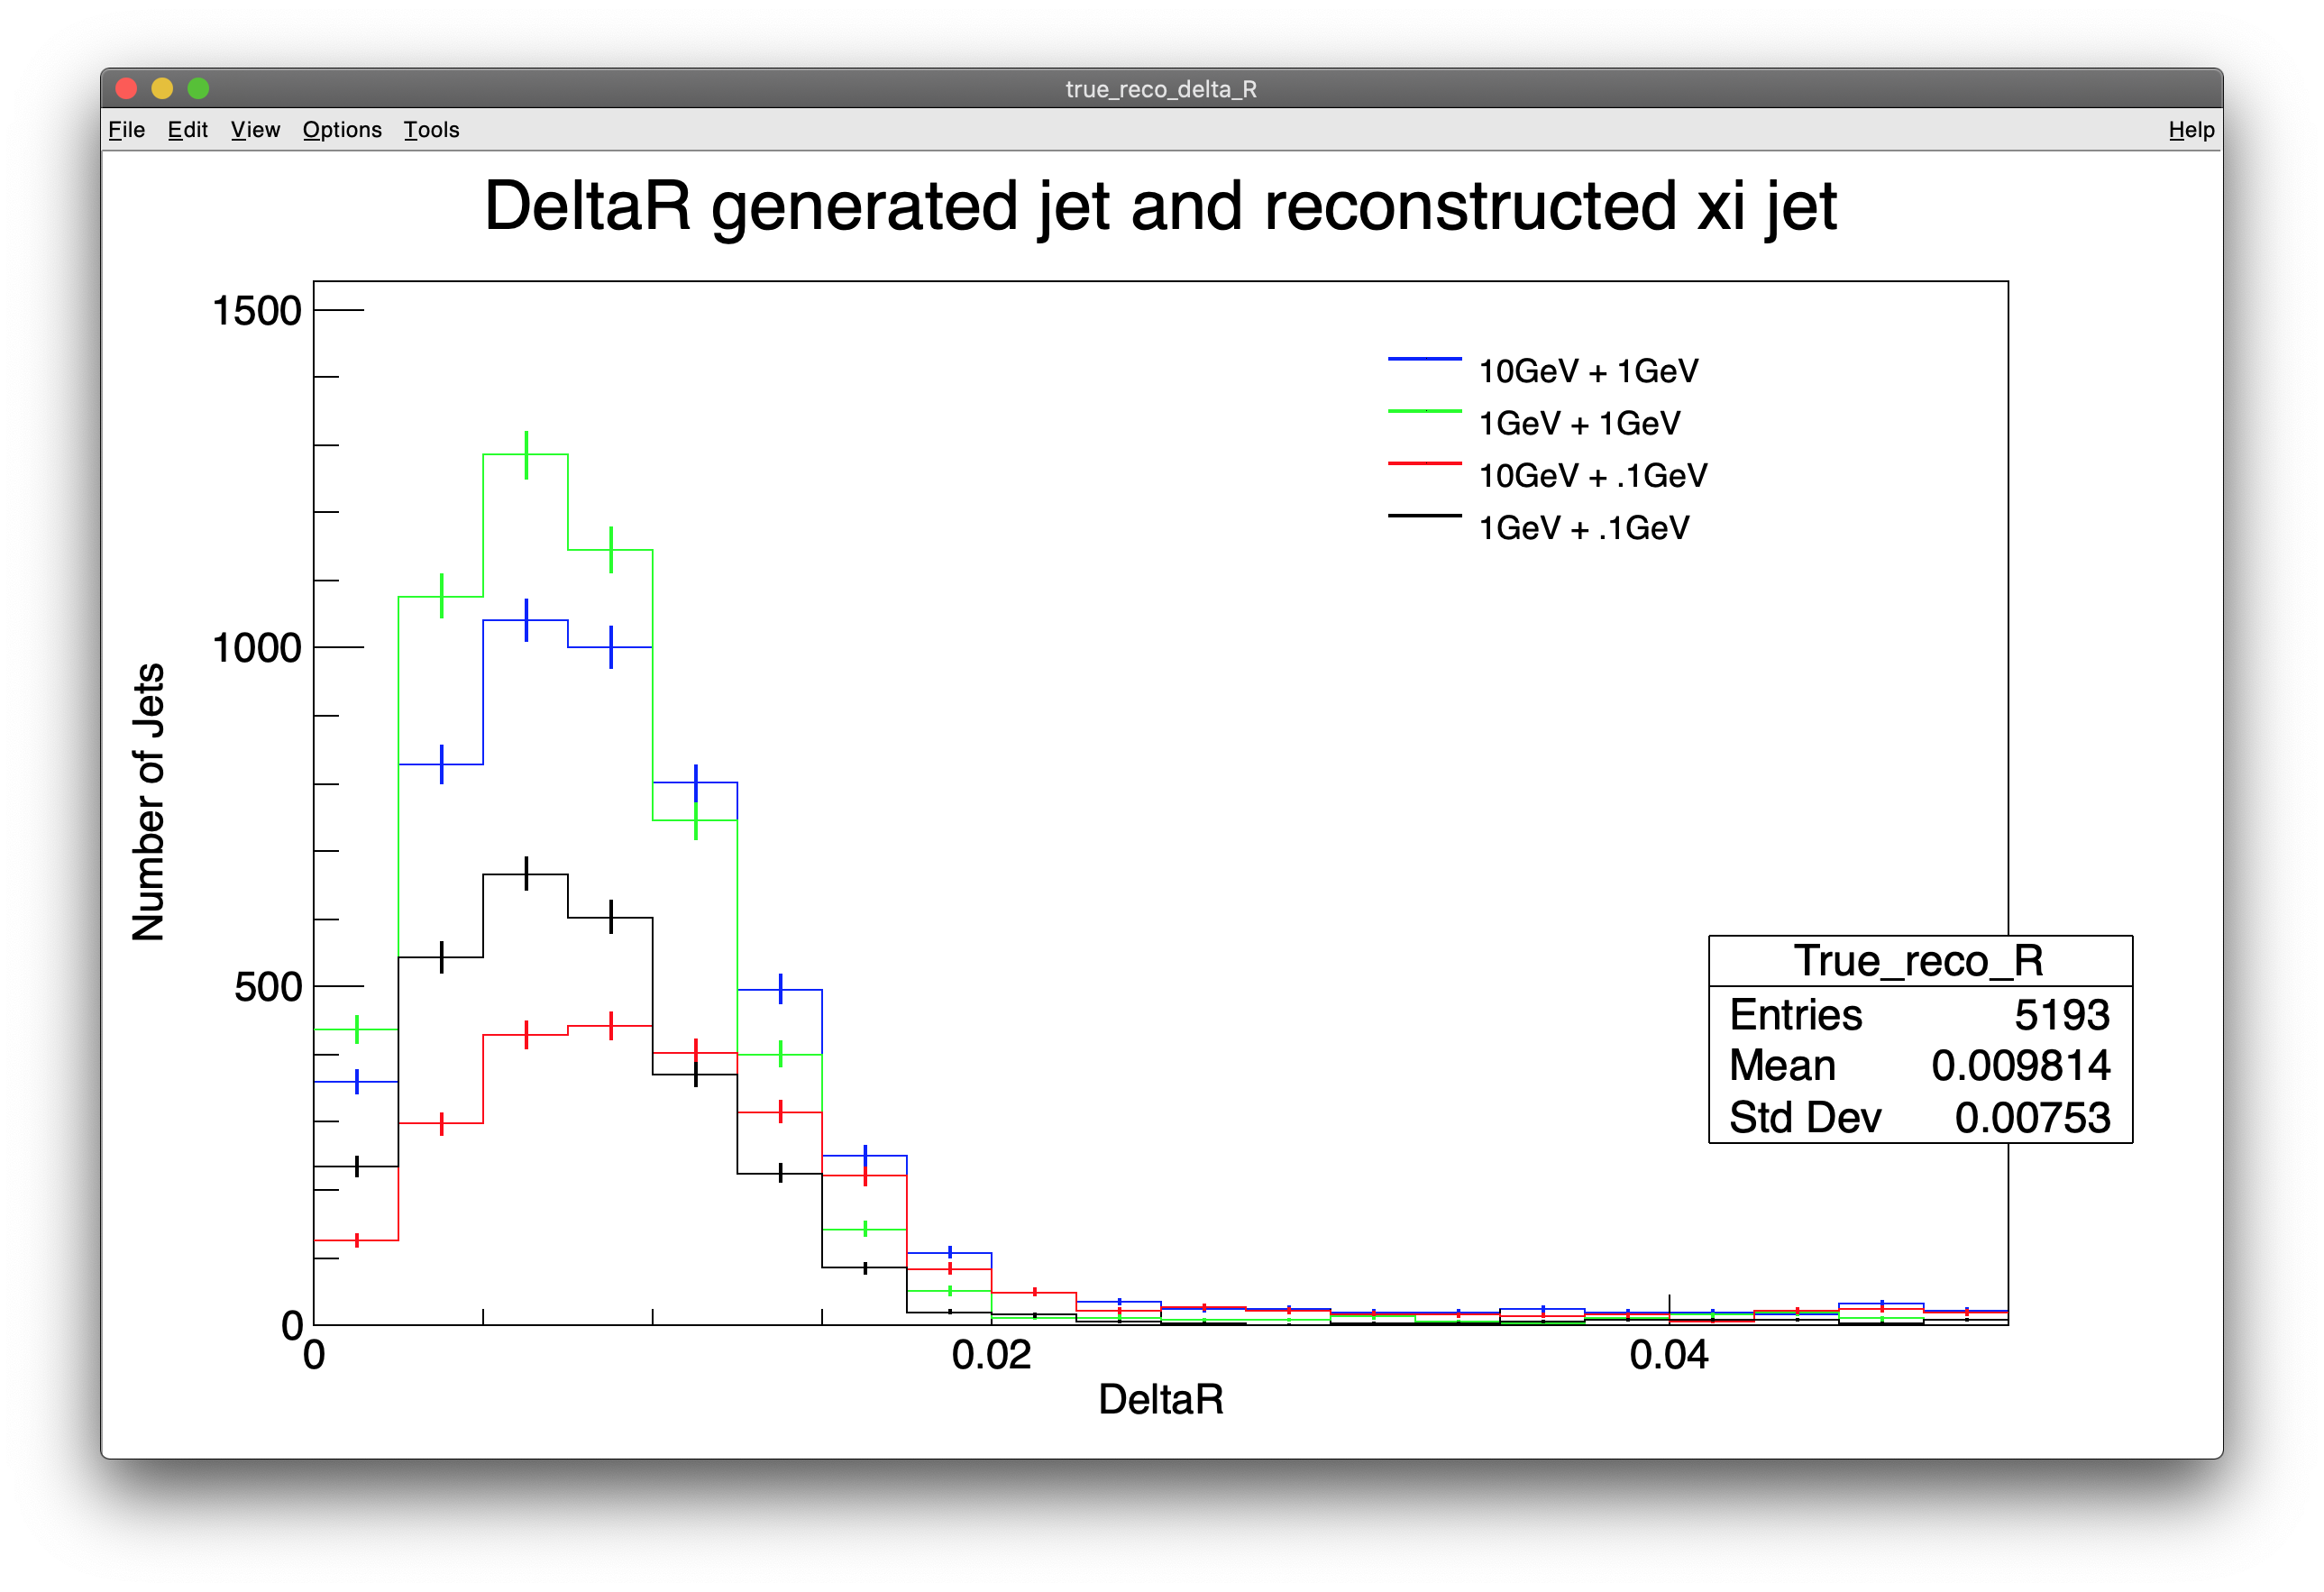
\includegraphics[width=13cm]{deltaR_gen_reco.png}

\caption{$\Delta R$ between reconstructed and generated xi jets. Distribution is independent of our model parameters showing good matching between the two.}
\label{fig:gen_reco}
\end{center}
\end{figure}

\begin{figure}[t]
\begin{center}
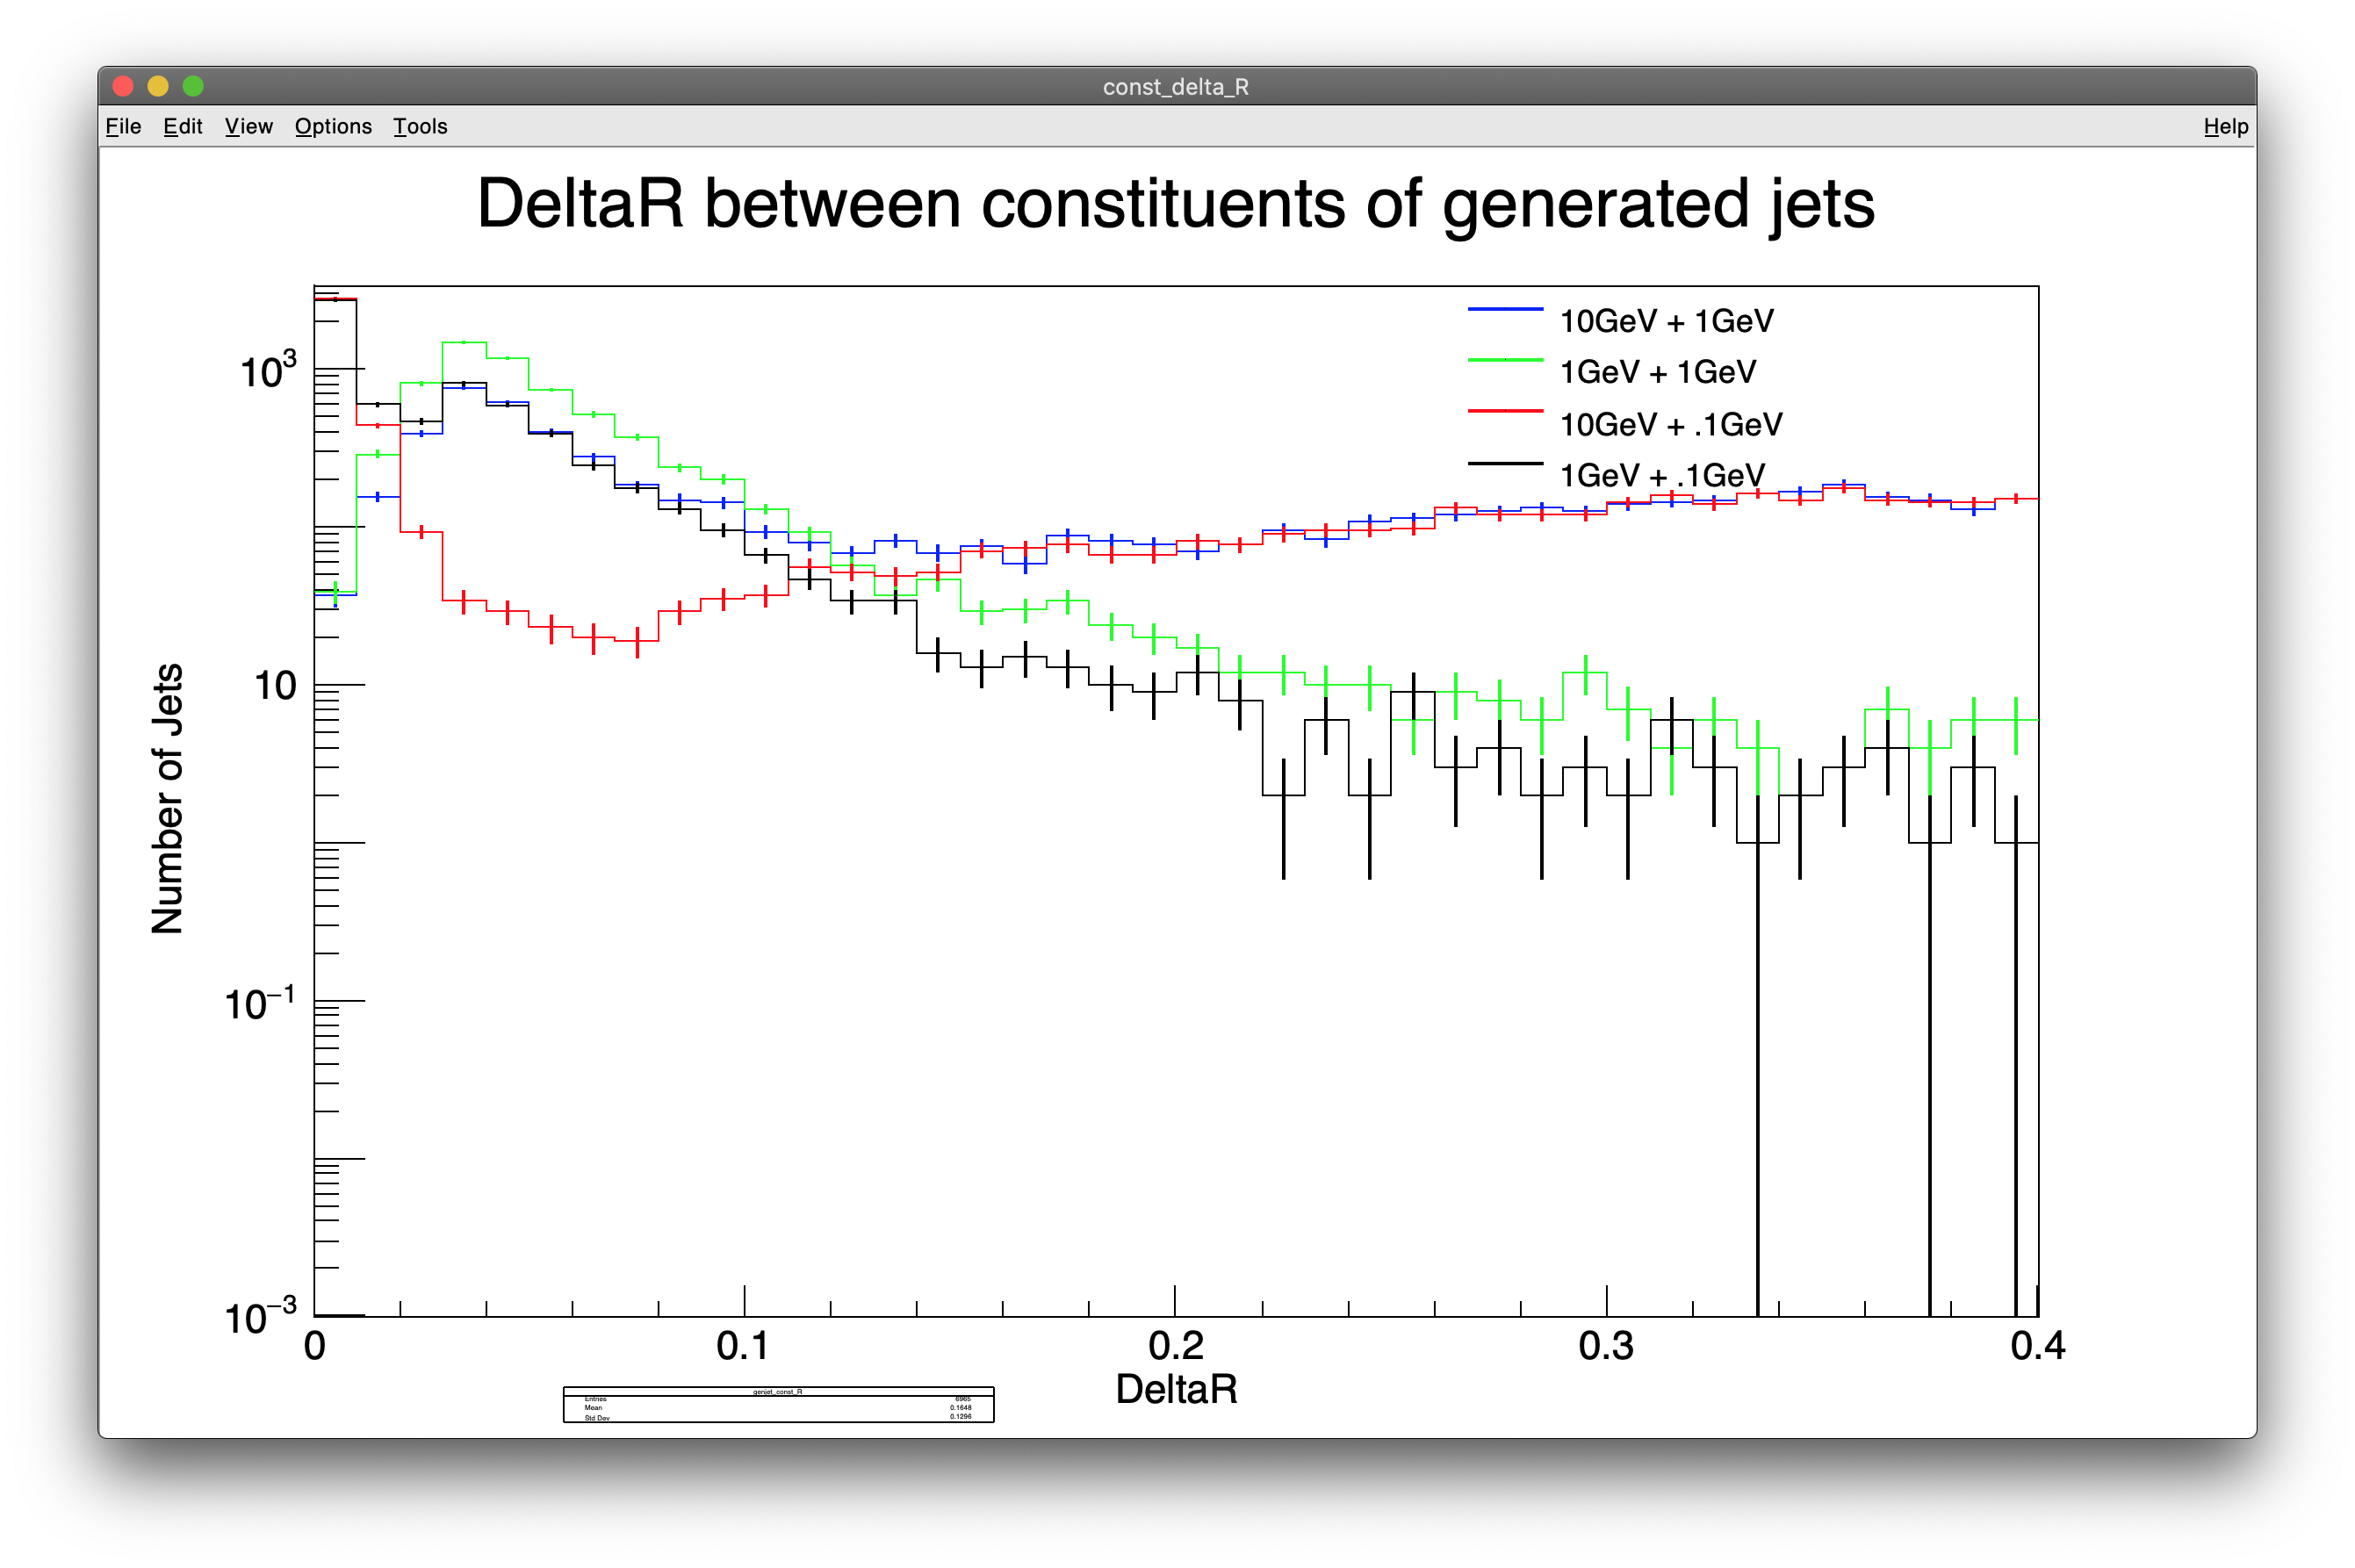
\includegraphics[width=13cm]{deltaR_const.png}

\caption{$\Delta R$ between constituents(photons) of our generated xi jets. Note the log scale. The long tails in the blue and red distributions are from the 10 GeV scalar which peaks at a $\Delta R$ of below 0.4. 1 GeV scalars peak at $\Delta R = 0.04$ and .01 GeV scalars peak well below $\Delta R = 0.025$ and would most likely be identified as single photons.}
\label{fig:const}
\end{center}
\end{figure}

For detail we show a number of additional plots which highlight the number of generated xi jets, reconstructed xi jets, matched reconstructed xi jets, and efficiency of xi jet reconstruction as a function of our scalar mass below. For these plots we produced 25000 events for each model point, where for each model we now only have 1 scalar with 1 mass, between 0.10 GeV and 10.0 GeV. 

\begin{figure}[t]
\begin{center}
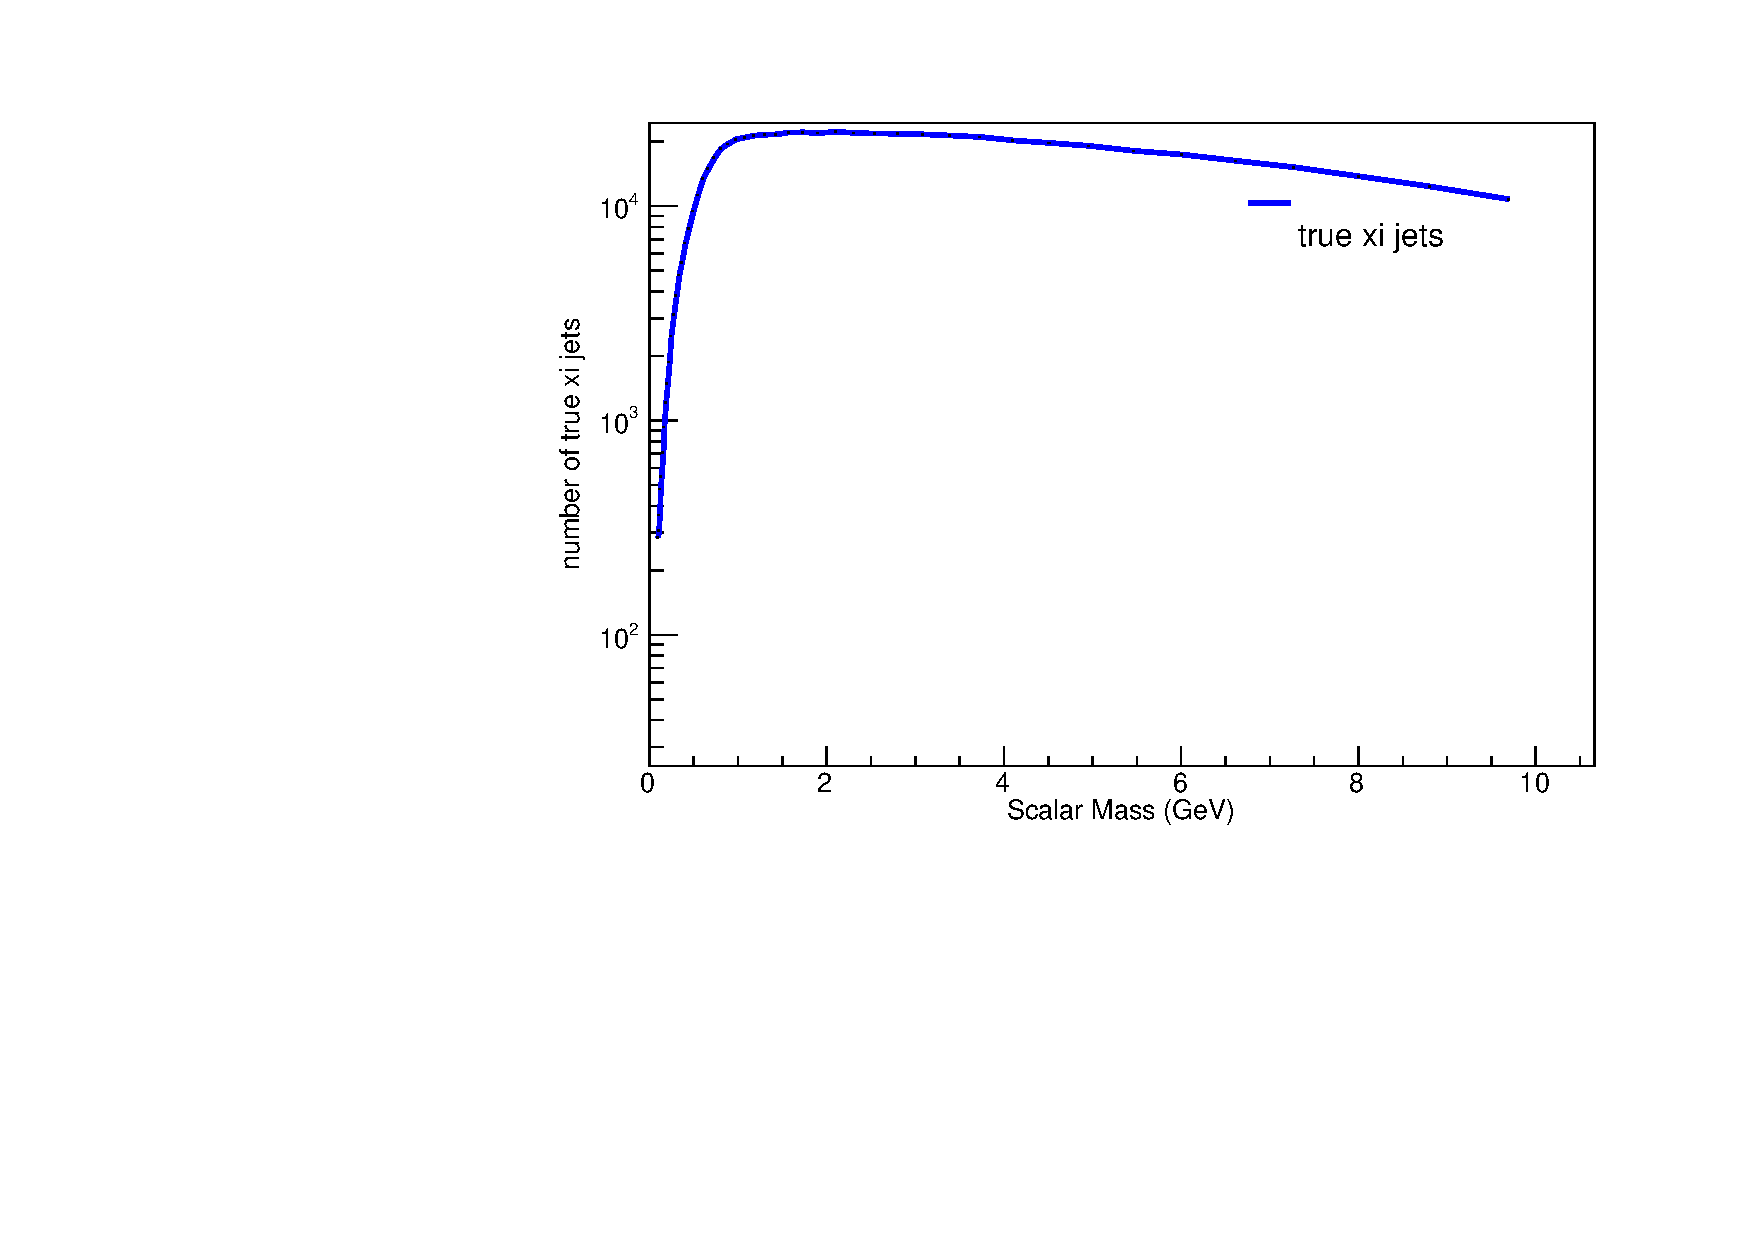
\includegraphics[width=10cm]{true_xi_jets.pdf}

\caption{Number of generated xi jets as a function of scalar mass. Note the log y axis. Total number of events for each point is 25000. At very low scalar masses, photons are highly collimated so few generated xi jets are found. This number rapidly climbs one $m_{\phi} = 1 GeV$.}
\label{default}
\end{center}
\end{figure}

\begin{figure}[t]
\begin{center}
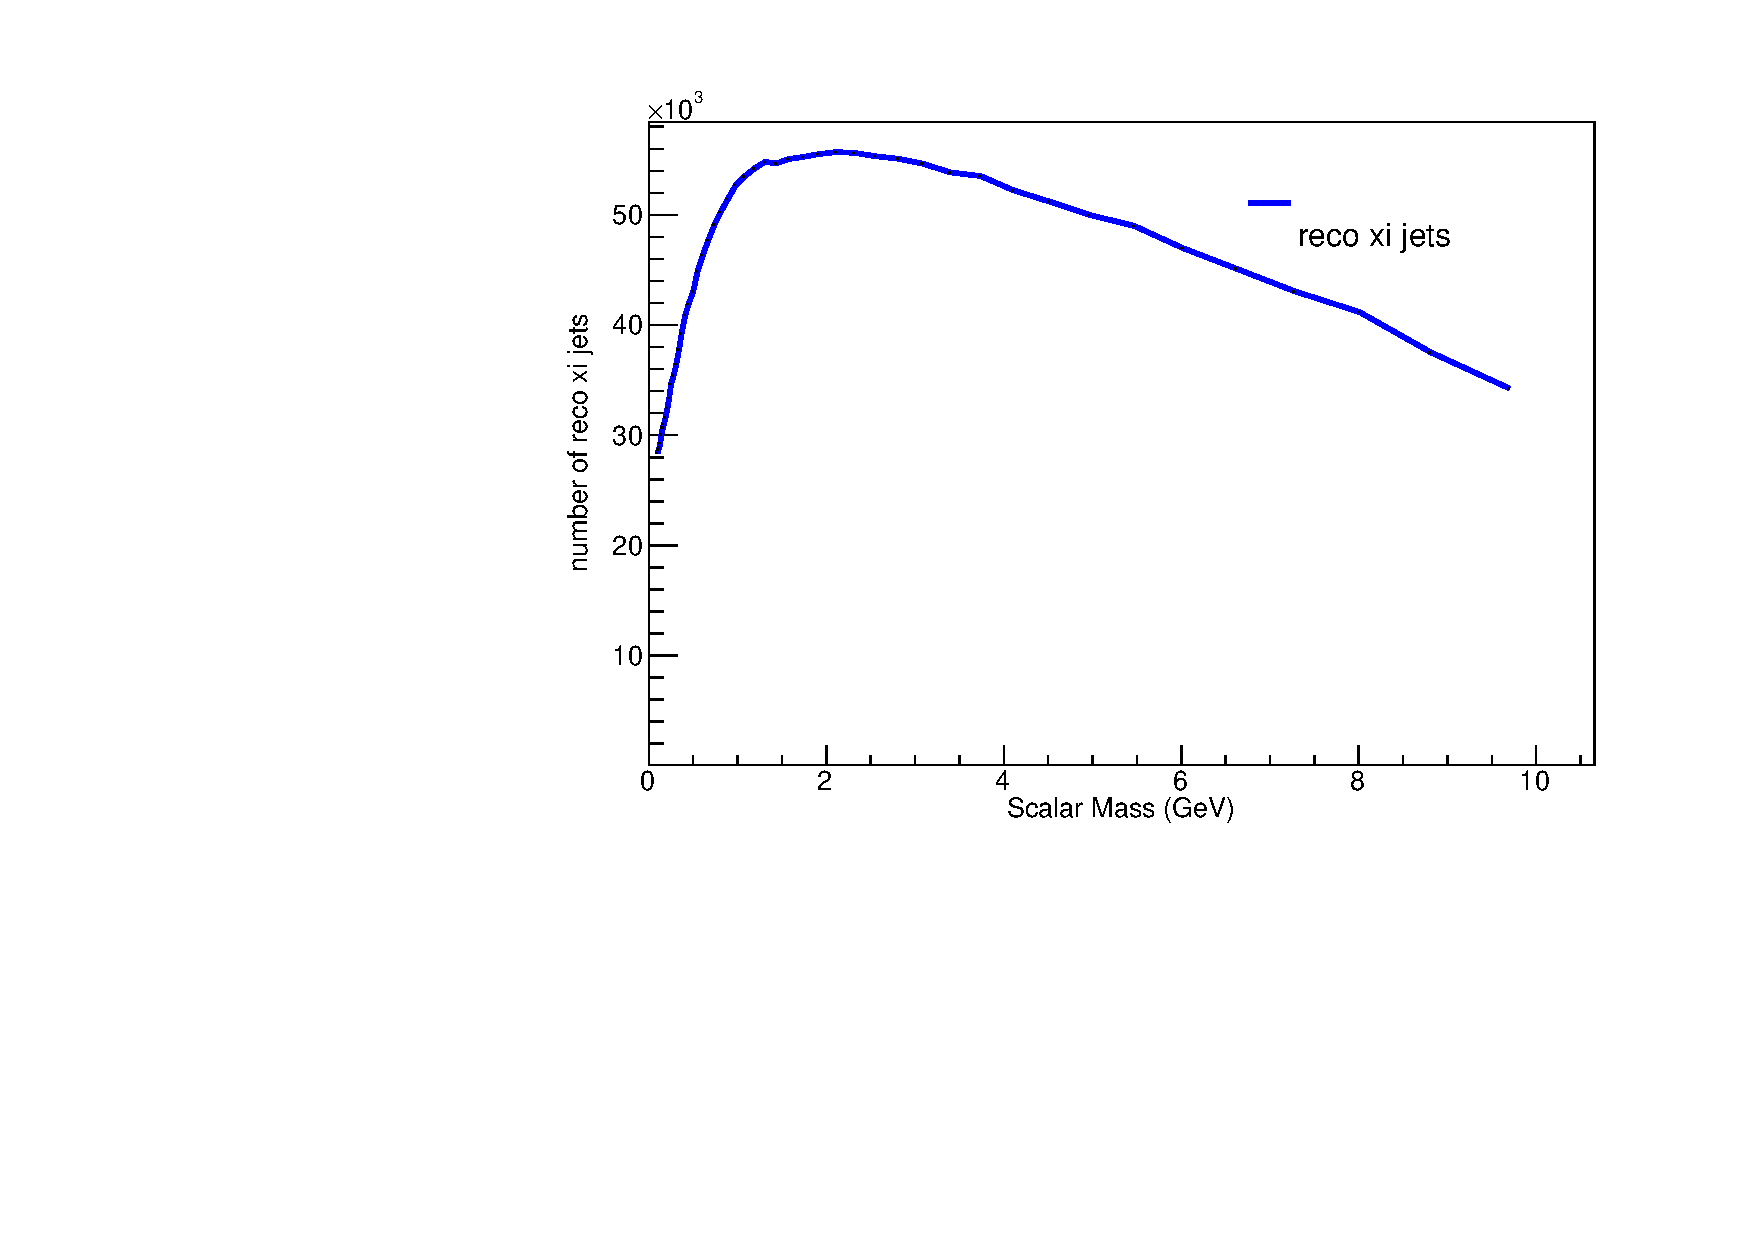
\includegraphics[width=10cm]{reco_xi_jets.pdf}

\caption{Number of reconstructed xi jets as a function of scalar mass. Total number of events for each point is 25000.}
\label{default}
\end{center}
\end{figure}

\begin{figure}[t]
\begin{center}
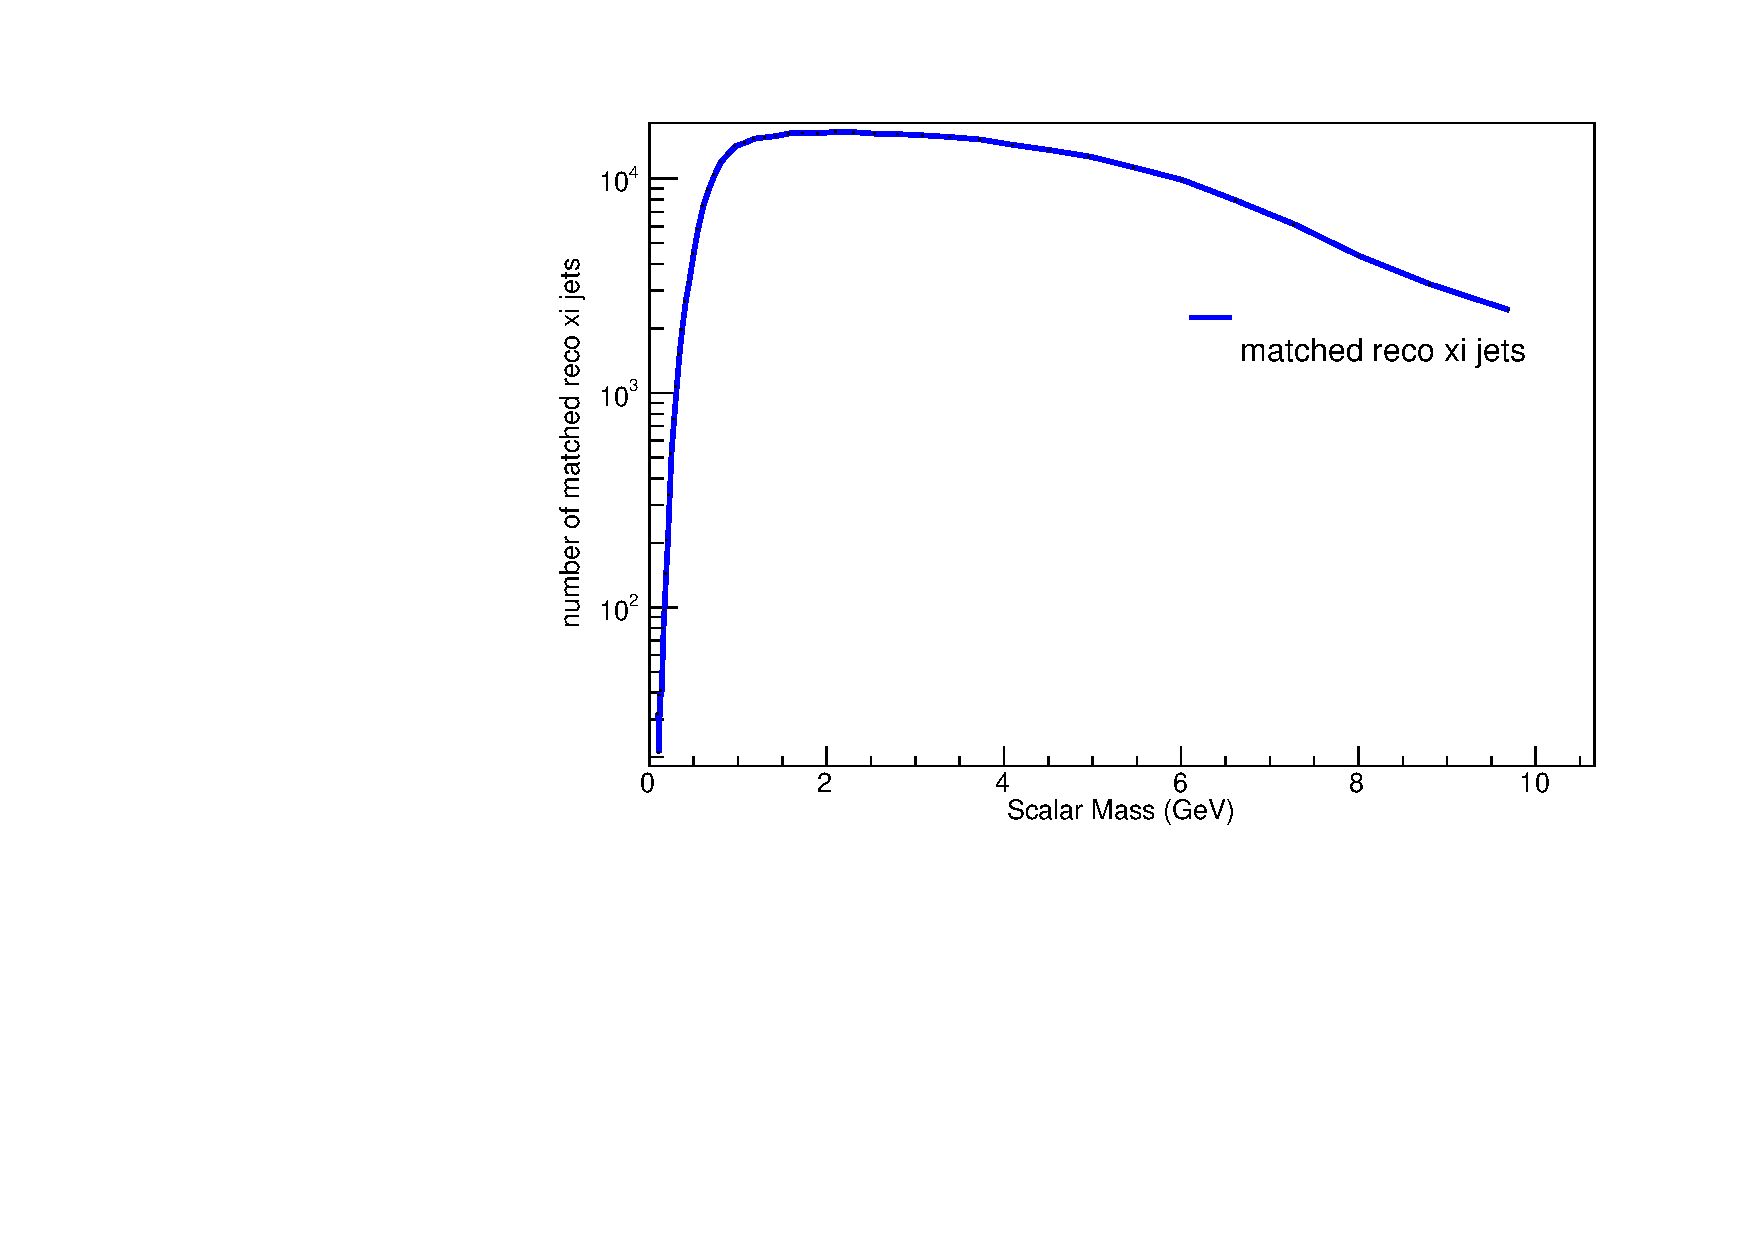
\includegraphics[width=10cm]{matched_reco_xi_jets.pdf}

\caption{Number of matched reconstructed xi jets as a function of scalar mass. Note the log y axis. Total number of events for each point is 25000. Again since the number of generated xi jets is extremely low for low scalar masses, the number of matched reconstructed jets is low as well.}
\label{default}
\end{center}
\end{figure}

\begin{figure}[t]
\begin{center}
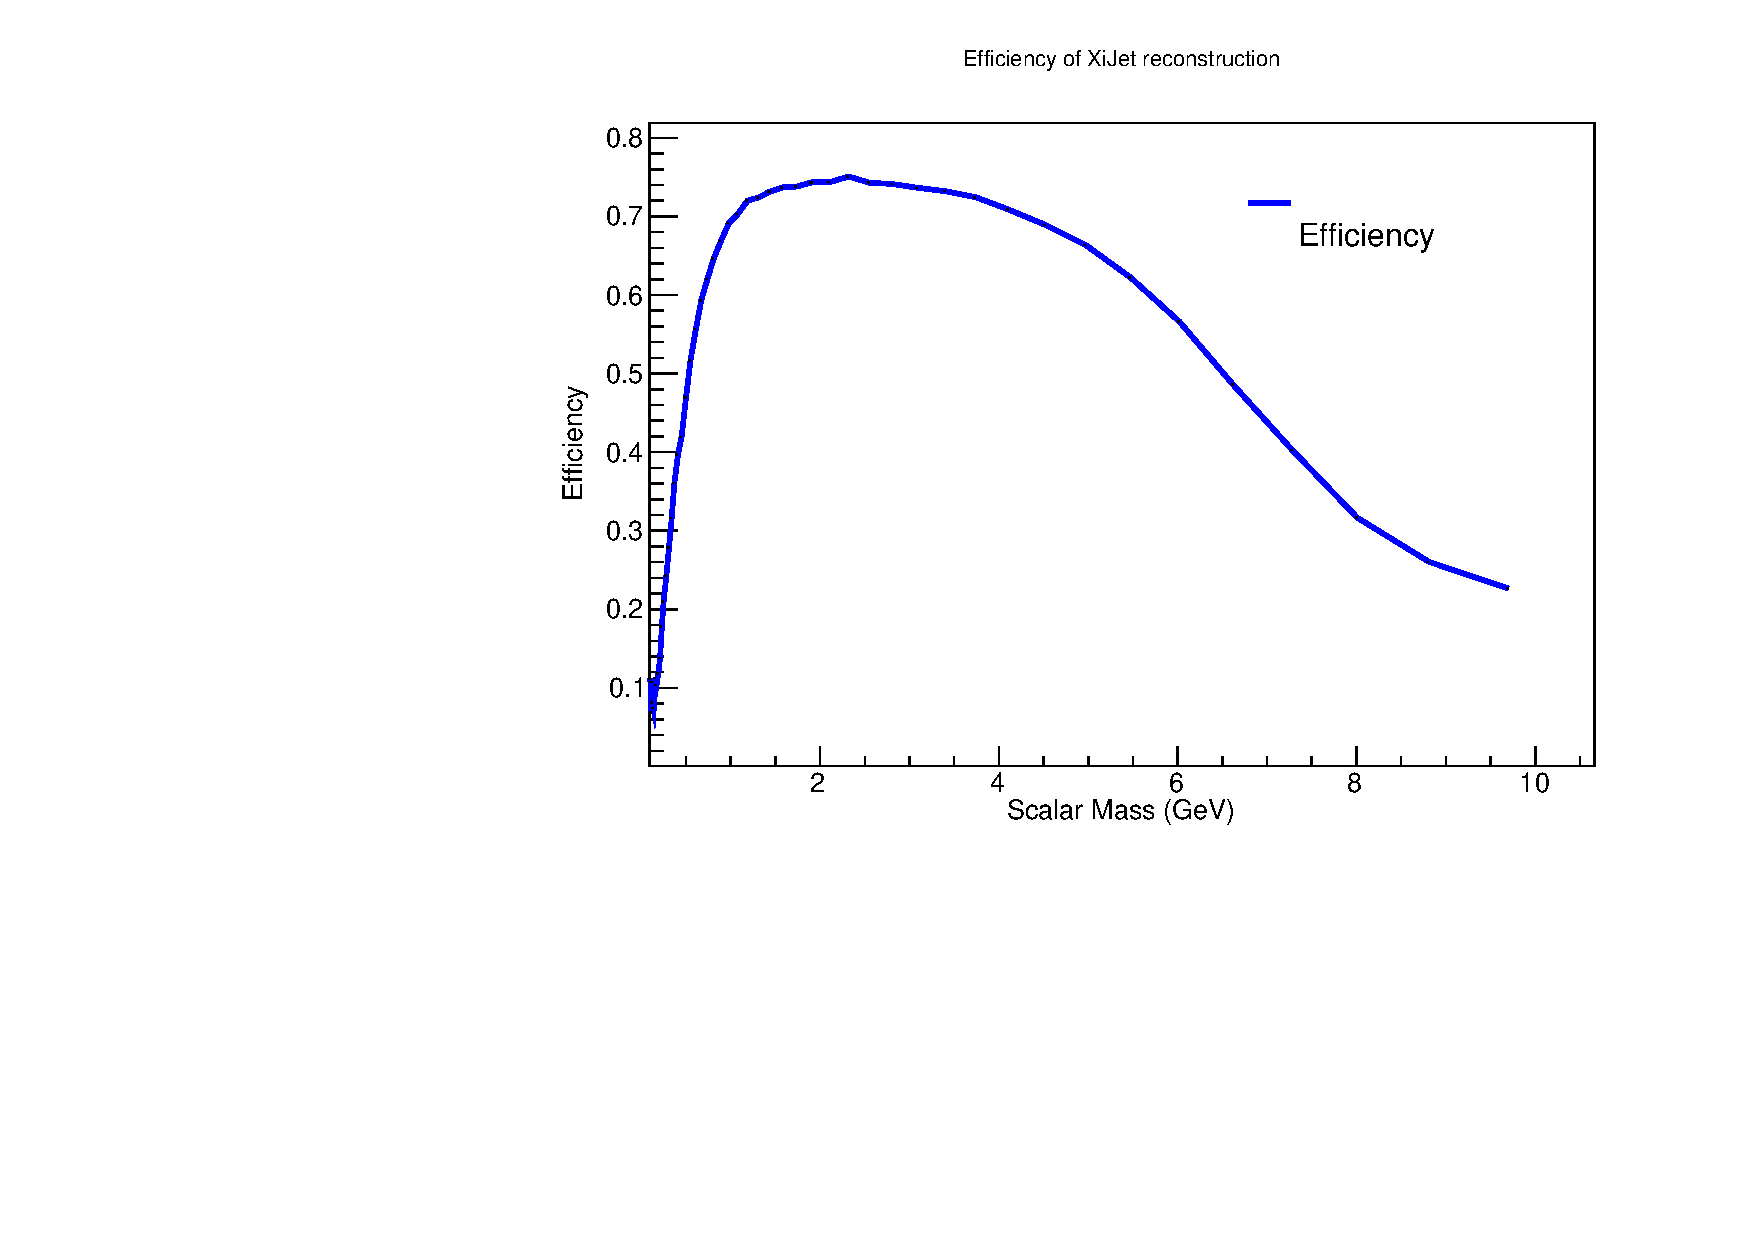
\includegraphics[width=10cm]{Efficiency.pdf}

\caption{Efficiency for generated xi jet reconstruction as a function of scalar mass. Efficiency peaks near 1.5 GeV and remains high until around 5 or 6 GeV. The tail at 10 GeV is around 25\% because the distribution of photon delta R's amongst photon pairs is quite wide, so xi jets with intermediate values of delta R are still produced.}
\label{default}
\end{center}
\end{figure}

\section{Reconstructing the Higgs}
Now we would like to understand how often we can reconstruct the higgs mass using our reconstructed photons and xi jets. To do so we first collect all of our reconstructed objects, which for now are photons and $\xi$ jets. We only require our reconstructed $\xi$ jets to pass our hadronic energy fraction cut, otherwise no cuts (besides minimum PT cuts which are used for clustering). We then form all the possible subsets of this collection, which have between 1 and 4 objects. The upper limit of 4 objects is because our scalar decays can result in at most 4 combinations of objects (either photons or $\xi$ jets).  If one combination of $\xi$ jets and photons yields an invariant mass within a 10 GeV window around $M_{125}$ ($115 GeV < M_{inv} < 135 GeV$) then we consider this a match. Virtually no events contain multiple combinations of photons and $\xi$ jets which satisfy this requirement. We further separate our sample to highlight the effect of turning on $\xi$ jet reconstruction as a function of scalar mass. We have several categories.

\begin{enumerate}
\item Photons only: 2, 3, or 4 photons reconstructing the higgs mass with no $\xi$ jets 
\item Photons + Xi jets: 1 $\xi$ + 1 photon, 2 $\xi$ + 1 photon, 1 $\xi$ + 2 photons
\item Xi jets inclusive: Same as Photons + Xi jets but adding 2 $\xi$ jets and no photons
\item Xi jets only: 2 $xi$ jets and no photons
\item All: Includes all above categories
\end{enumerate}

One can see in Fig.~\ref{fig:higgs_reco_eff} that the efficiency for reconstructing higgs events with only photons in this scalar mass range is quite low, peaking at very low and very high scalar masses. Adding photons + $\xi$ jets (as explained above) increases the efficiency moderately at intermediate scalar masses. The real payoff comes from adding the $\xi$ jet only category (cyan) for which the efficiency peaks between 1 and 7 GeV. Below 1 GeV and above 7 GeV this efficiency drops below the photon only efficiency because the photons are either well collimated (the former case) or well separated (the latter case) and thus are identified as single photons and not as $\xi$ jets. 

\begin{figure}[t]
\begin{center}
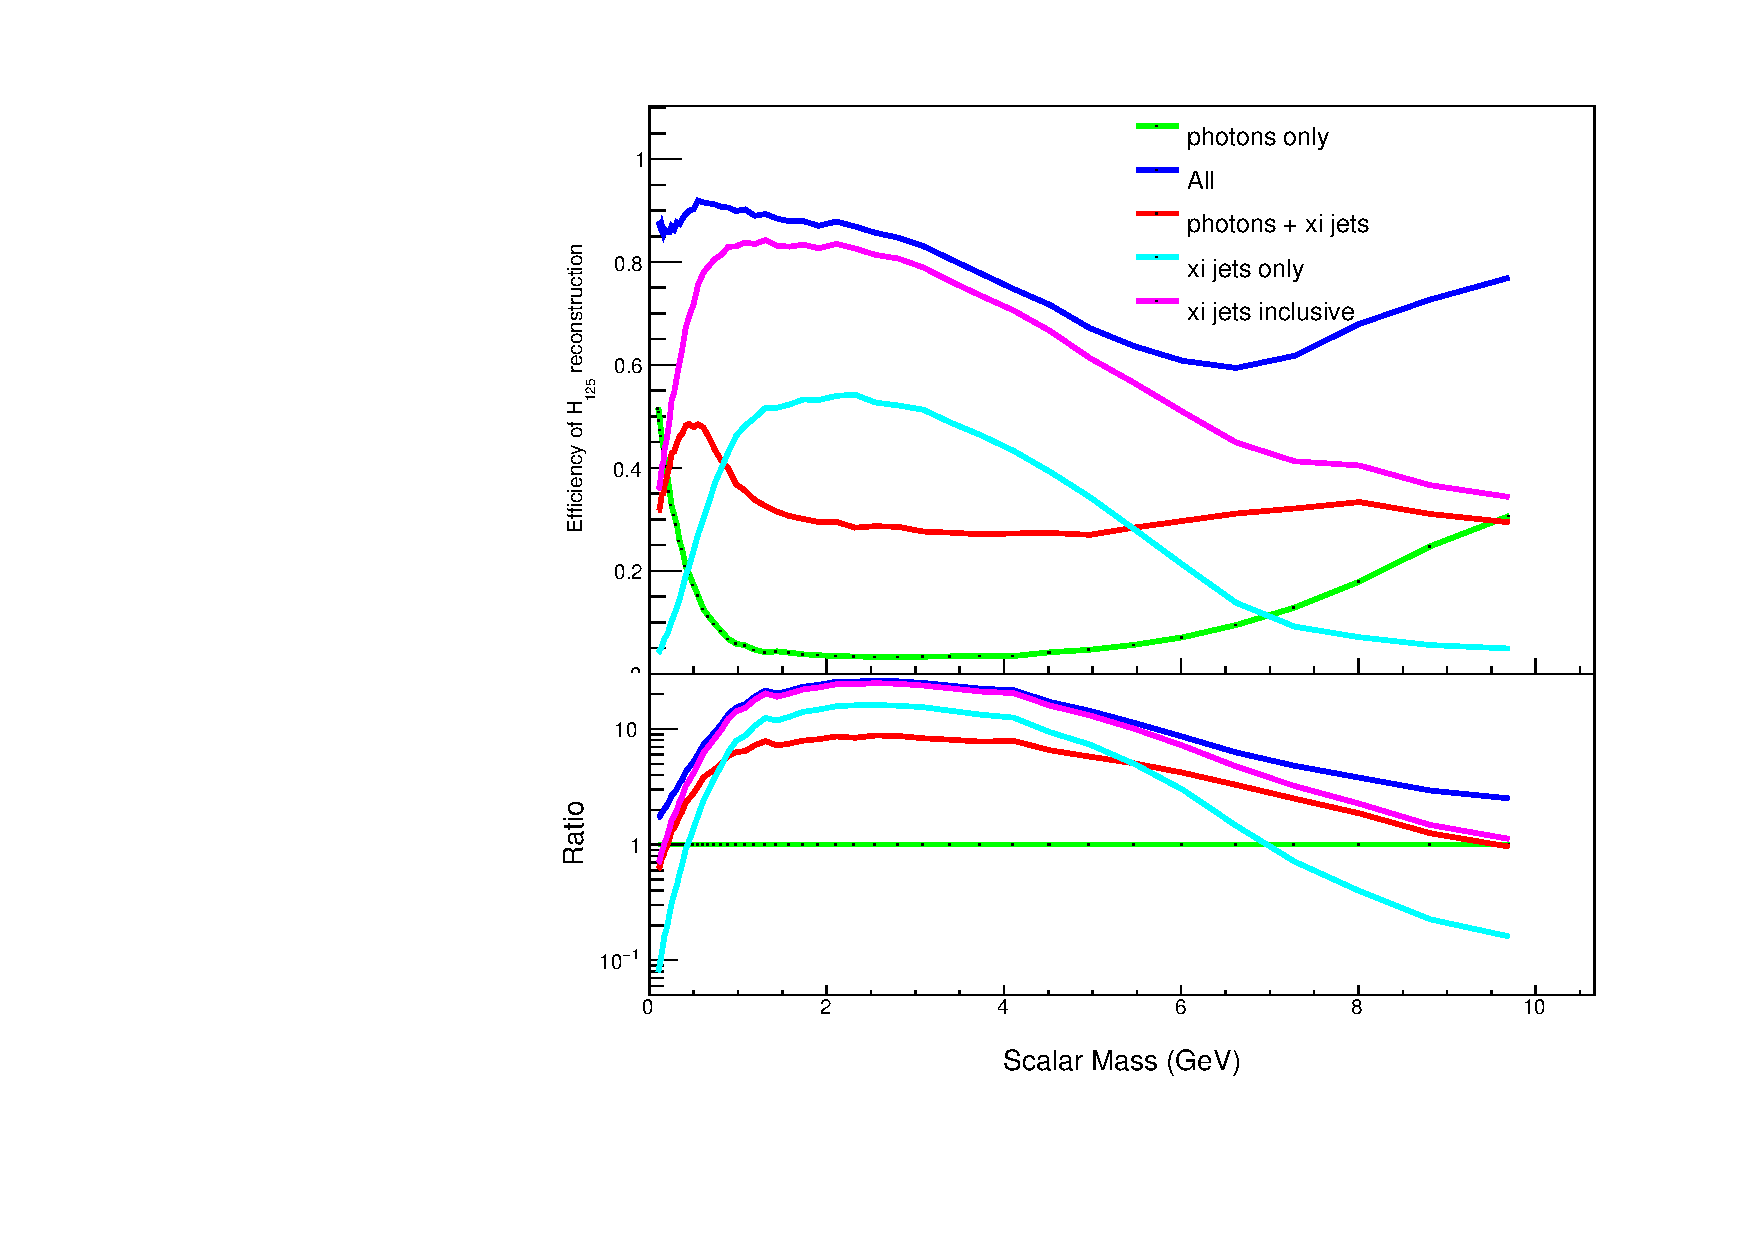
\includegraphics[width=12cm]{higgs_reco_eff.pdf}

\caption{Top: Number of reconstructed $H_{125}$ as a function of scalar mass using only photons(green), photons + $\xi$ jets(red), $\xi$ jets only(cyan), $\xi$ jets inclusive(purple), and all categories(blue.)  Bottom: Ratio to photons only.  the efficiency for reconstructing higgs events with only photons in this scalar mass range is quite low, peaking at very low and very high scalar masses. Adding photons + $\xi$ jets (as explained above) increases the efficiency moderately at intermediate scalar masses. The real payoff comes from adding the $\xi$ jet only category (cyan) for which the efficiency peaks between 1 and 7 GeV. Below 1 GeV and above 7 GeV this efficiency drops below the photon only efficiency because the photons are either well collimated (the former case) or well separated (the latter case) and thus are identified as single photons and not as $\xi$ jets.}
\label{fig:higgs_reco_eff}
\end{center}
\end{figure}


\bibliographystyle{utphys}
\bibliography{update_noah}

\end{document}